
\documentclass[a4paper,UKenglish,cleveref, autoref, thm-restate]{lipics-v2021}
%This is a template for producing LIPIcs articles. 
%See lipics-v2021-authors-guidelines.pdf for further information.
%for A4 paper format use option "a4paper", for US-letter use option "letterpaper"
%for british hyphenation rules use option "UKenglish", for american hyphenation rules use option "USenglish"
%for section-numbered lemmas etc., use "numberwithinsect"
%for enabling cleveref support, use "cleveref"
%for enabling autoref support, use "autoref"
%for anonymousing the authors (e.g. for double-blind review), add "anonymous"
%for enabling thm-restate support, use "thm-restate"
%for enabling a two-column layout for the author/affilation part (only applicable for > 6 authors), use "authorcolumns"
%for producing a PDF according the PDF/A standard, add "pdfa"

\pdfoutput=1 %uncomment to ensure pdflatex processing (mandatatory e.g. to submit to arXiv)
%\hideLIPIcs  %uncomment to remove references to LIPIcs series (logo, DOI, ...), e.g. when preparing a pre-final version to be uploaded to arXiv or another public repository

%\graphicspath{{./graphics/}}%helpful if your graphic files are in another directory

\bibliographystyle{plainurl}% the mandatory bibstyle

\title{Universality Frontier for Asynchronous Cellular Automata} 

%\titlerunning{} %TODO optional, please use if title is longer than one line

\author{Ivan Baburin}{Department of Computer Science,
  ETH Z{\"u}rich, Switzerland}{ivan.baburin@inf.ethz.ch}{}{}%TODO mandatory, please use full name; only 1 author per \author macro; first two parameters are mandatory, other parameters can be empty. Please provide at least the name of the affiliation and the country. The full address is optional. Use additional curly braces to indicate the correct name splitting when the last name consists of multiple name parts.
  
\author{Matthew Cook}{Faculty of Science and Engineering,
  University of Groningen}{cook@ini.ethz.ch}{}{}

\author{Florian Grötschla}{Department of Electrical Engineering,
  ETH Z{\"u}rich, Switzerland}{fgroetschla@ethz.ch}{}{}

\author{Andreas Plesner}{Department of Electrical Engineering,
  ETH Z{\"u}rich, Switzerland}{aplesner@ethz.ch}{}{}

\author{Roger Wattenhofer}{Department of Electrical Engineering,
  ETH Z{\"u}rich, Switzerland}{wattenhofer@ethz.ch}{}{}

\authorrunning{I. Baburin et al.} %TODO mandatory. First: Use abbreviated first/middle names. Second (only in severe cases): Use first author plus 'et al.'

\Copyright{Ivan Baburin, Matthew Cook, Florian Grötschla, Andreas Plesner, Roger Wattenhofer} %TODO mandatory, please use full first names. LIPIcs license is "CC-BY";  http://creativecommons.org/licenses/by/3.0/

% uncomment for anonymous submission
% \author{Submission 105}{ICALP 2025}{}{}{}
% \authorrunning{Submission ??}
% \Copyright{Submission ??}


\begin{CCSXML}
<ccs2012>
   <concept>
       <concept_id>10003752.10003753</concept_id>
       <concept_desc>Theory of computation~Models of computation</concept_desc>
       <concept_significance>300</concept_significance>
       </concept>
 </ccs2012>
\end{CCSXML}

\ccsdesc[300]{Theory of computation~Models of computation}
%TODO mandatory: Please choose ACM 2012 classifications from https://dl.acm.org/ccs/ccs_flat.cfm 

\keywords{Universality, Cellular Automata, Automata Networks, Asynchronous updating} %TODO mandatory; please add comma-separated list of keywords

%\category{} %optional, e.g. invited paper

%\relatedversion{} %optional, e.g. full version hosted on arXiv, HAL, or other respository/website
%\relatedversiondetails[linktext={opt. text shown instead of the URL}, cite=DBLP:books/mk/GrayR93]{Classification (e.g. Full Version, Extended Version, Previous Version}{URL to related version} %linktext and cite are optional

%\supplement{}%optional, e.g. related research data, source code, ... hosted on a repository like zenodo, figshare, GitHub, ...
%\supplementdetails[linktext={opt. text shown instead of the URL}, cite=DBLP:books/mk/GrayR93, subcategory={Description, Subcategory}, swhid={Software Heritage Identifier}]{General Classification (e.g. Software, Dataset, Model, ...)}{URL to related version} %linktext, cite, and subcategory are optional

%\funding{(Optional) general funding statement \dots}%optional, to capture a funding statement, which applies to all authors. Please enter author specific funding statements as fifth argument of the \author macro.

%\acknowledgements{I want to thank \dots}%optional

\nolinenumbers %uncomment to disable line numbering


%Editor-only macros:: begin (do not touch as author)%%%%%%%%%%%%%%%%%%%%%%%%%%%%%%%%%%
\EventEditors{John Q. Open and Joan R. Access}
\EventNoEds{2}
\EventLongTitle{42nd Conference on Very Important Topics (CVIT 2016)}
\EventShortTitle{CVIT 2016}
\EventAcronym{CVIT}
\EventYear{2016}
\EventDate{December 24--27, 2016}
\EventLocation{Little Whinging, United Kingdom}
\EventLogo{}
\SeriesVolume{42}
\ArticleNo{23}
%%%%%%%%%%%%%%%%%%%%%%%%%%%%%%%%%%%%%%%%%%%%%%%%%%%%%%


%
\setlength\unitlength{1mm}
\newcommand{\twodots}{\mathinner {\ldotp \ldotp}}
% bb font symbols
\newcommand{\Rho}{\mathrm{P}}
\newcommand{\Tau}{\mathrm{T}}

\newfont{\bbb}{msbm10 scaled 700}
\newcommand{\CCC}{\mbox{\bbb C}}

\newfont{\bb}{msbm10 scaled 1100}
\newcommand{\CC}{\mbox{\bb C}}
\newcommand{\PP}{\mbox{\bb P}}
\newcommand{\RR}{\mbox{\bb R}}
\newcommand{\QQ}{\mbox{\bb Q}}
\newcommand{\ZZ}{\mbox{\bb Z}}
\newcommand{\FF}{\mbox{\bb F}}
\newcommand{\GG}{\mbox{\bb G}}
\newcommand{\EE}{\mbox{\bb E}}
\newcommand{\NN}{\mbox{\bb N}}
\newcommand{\KK}{\mbox{\bb K}}
\newcommand{\HH}{\mbox{\bb H}}
\newcommand{\SSS}{\mbox{\bb S}}
\newcommand{\UU}{\mbox{\bb U}}
\newcommand{\VV}{\mbox{\bb V}}


\newcommand{\yy}{\mathbbm{y}}
\newcommand{\xx}{\mathbbm{x}}
\newcommand{\zz}{\mathbbm{z}}
\newcommand{\sss}{\mathbbm{s}}
\newcommand{\rr}{\mathbbm{r}}
\newcommand{\pp}{\mathbbm{p}}
\newcommand{\qq}{\mathbbm{q}}
\newcommand{\ww}{\mathbbm{w}}
\newcommand{\hh}{\mathbbm{h}}
\newcommand{\vvv}{\mathbbm{v}}

% Vectors

\newcommand{\av}{{\bf a}}
\newcommand{\bv}{{\bf b}}
\newcommand{\cv}{{\bf c}}
\newcommand{\dv}{{\bf d}}
\newcommand{\ev}{{\bf e}}
\newcommand{\fv}{{\bf f}}
\newcommand{\gv}{{\bf g}}
\newcommand{\hv}{{\bf h}}
\newcommand{\iv}{{\bf i}}
\newcommand{\jv}{{\bf j}}
\newcommand{\kv}{{\bf k}}
\newcommand{\lv}{{\bf l}}
\newcommand{\mv}{{\bf m}}
\newcommand{\nv}{{\bf n}}
\newcommand{\ov}{{\bf o}}
\newcommand{\pv}{{\bf p}}
\newcommand{\qv}{{\bf q}}
\newcommand{\rv}{{\bf r}}
\newcommand{\sv}{{\bf s}}
\newcommand{\tv}{{\bf t}}
\newcommand{\uv}{{\bf u}}
\newcommand{\wv}{{\bf w}}
\newcommand{\vv}{{\bf v}}
\newcommand{\xv}{{\bf x}}
\newcommand{\yv}{{\bf y}}
\newcommand{\zv}{{\bf z}}
\newcommand{\zerov}{{\bf 0}}
\newcommand{\onev}{{\bf 1}}

% Matrices

\newcommand{\Am}{{\bf A}}
\newcommand{\Bm}{{\bf B}}
\newcommand{\Cm}{{\bf C}}
\newcommand{\Dm}{{\bf D}}
\newcommand{\Em}{{\bf E}}
\newcommand{\Fm}{{\bf F}}
\newcommand{\Gm}{{\bf G}}
\newcommand{\Hm}{{\bf H}}
\newcommand{\Id}{{\bf I}}
\newcommand{\Jm}{{\bf J}}
\newcommand{\Km}{{\bf K}}
\newcommand{\Lm}{{\bf L}}
\newcommand{\Mm}{{\bf M}}
\newcommand{\Nm}{{\bf N}}
\newcommand{\Om}{{\bf O}}
\newcommand{\Pm}{{\bf P}}
\newcommand{\Qm}{{\bf Q}}
\newcommand{\Rm}{{\bf R}}
\newcommand{\Sm}{{\bf S}}
\newcommand{\Tm}{{\bf T}}
\newcommand{\Um}{{\bf U}}
\newcommand{\Wm}{{\bf W}}
\newcommand{\Vm}{{\bf V}}
\newcommand{\Xm}{{\bf X}}
\newcommand{\Ym}{{\bf Y}}
\newcommand{\Zm}{{\bf Z}}

% Calligraphic

\newcommand{\Ac}{{\cal A}}
\newcommand{\Bc}{{\cal B}}
\newcommand{\Cc}{{\cal C}}
\newcommand{\Dc}{{\cal D}}
\newcommand{\Ec}{{\cal E}}
\newcommand{\Fc}{{\cal F}}
\newcommand{\Gc}{{\cal G}}
\newcommand{\Hc}{{\cal H}}
\newcommand{\Ic}{{\cal I}}
\newcommand{\Jc}{{\cal J}}
\newcommand{\Kc}{{\cal K}}
\newcommand{\Lc}{{\cal L}}
\newcommand{\Mc}{{\cal M}}
\newcommand{\Nc}{{\cal N}}
\newcommand{\nc}{{\cal n}}
\newcommand{\Oc}{{\cal O}}
\newcommand{\Pc}{{\cal P}}
\newcommand{\Qc}{{\cal Q}}
\newcommand{\Rc}{{\cal R}}
\newcommand{\Sc}{{\cal S}}
\newcommand{\Tc}{{\cal T}}
\newcommand{\Uc}{{\cal U}}
\newcommand{\Wc}{{\cal W}}
\newcommand{\Vc}{{\cal V}}
\newcommand{\Xc}{{\cal X}}
\newcommand{\Yc}{{\cal Y}}
\newcommand{\Zc}{{\cal Z}}

% Bold greek letters

\newcommand{\alphav}{\hbox{\boldmath$\alpha$}}
\newcommand{\betav}{\hbox{\boldmath$\beta$}}
\newcommand{\gammav}{\hbox{\boldmath$\gamma$}}
\newcommand{\deltav}{\hbox{\boldmath$\delta$}}
\newcommand{\etav}{\hbox{\boldmath$\eta$}}
\newcommand{\lambdav}{\hbox{\boldmath$\lambda$}}
\newcommand{\epsilonv}{\hbox{\boldmath$\epsilon$}}
\newcommand{\nuv}{\hbox{\boldmath$\nu$}}
\newcommand{\muv}{\hbox{\boldmath$\mu$}}
\newcommand{\zetav}{\hbox{\boldmath$\zeta$}}
\newcommand{\phiv}{\hbox{\boldmath$\phi$}}
\newcommand{\psiv}{\hbox{\boldmath$\psi$}}
\newcommand{\thetav}{\hbox{\boldmath$\theta$}}
\newcommand{\tauv}{\hbox{\boldmath$\tau$}}
\newcommand{\omegav}{\hbox{\boldmath$\omega$}}
\newcommand{\xiv}{\hbox{\boldmath$\xi$}}
\newcommand{\sigmav}{\hbox{\boldmath$\sigma$}}
\newcommand{\piv}{\hbox{\boldmath$\pi$}}
\newcommand{\rhov}{\hbox{\boldmath$\rho$}}
\newcommand{\upsilonv}{\hbox{\boldmath$\upsilon$}}

\newcommand{\Gammam}{\hbox{\boldmath$\Gamma$}}
\newcommand{\Lambdam}{\hbox{\boldmath$\Lambda$}}
\newcommand{\Deltam}{\hbox{\boldmath$\Delta$}}
\newcommand{\Sigmam}{\hbox{\boldmath$\Sigma$}}
\newcommand{\Phim}{\hbox{\boldmath$\Phi$}}
\newcommand{\Pim}{\hbox{\boldmath$\Pi$}}
\newcommand{\Psim}{\hbox{\boldmath$\Psi$}}
\newcommand{\Thetam}{\hbox{\boldmath$\Theta$}}
\newcommand{\Omegam}{\hbox{\boldmath$\Omega$}}
\newcommand{\Xim}{\hbox{\boldmath$\Xi$}}


% Sans Serif small case

\newcommand{\Gsf}{{\sf G}}

\newcommand{\asf}{{\sf a}}
\newcommand{\bsf}{{\sf b}}
\newcommand{\csf}{{\sf c}}
\newcommand{\dsf}{{\sf d}}
\newcommand{\esf}{{\sf e}}
\newcommand{\fsf}{{\sf f}}
\newcommand{\gsf}{{\sf g}}
\newcommand{\hsf}{{\sf h}}
\newcommand{\isf}{{\sf i}}
\newcommand{\jsf}{{\sf j}}
\newcommand{\ksf}{{\sf k}}
\newcommand{\lsf}{{\sf l}}
\newcommand{\msf}{{\sf m}}
\newcommand{\nsf}{{\sf n}}
\newcommand{\osf}{{\sf o}}
\newcommand{\psf}{{\sf p}}
\newcommand{\qsf}{{\sf q}}
\newcommand{\rsf}{{\sf r}}
\newcommand{\ssf}{{\sf s}}
\newcommand{\tsf}{{\sf t}}
\newcommand{\usf}{{\sf u}}
\newcommand{\wsf}{{\sf w}}
\newcommand{\vsf}{{\sf v}}
\newcommand{\xsf}{{\sf x}}
\newcommand{\ysf}{{\sf y}}
\newcommand{\zsf}{{\sf z}}


% mixed symbols

\newcommand{\sinc}{{\hbox{sinc}}}
\newcommand{\diag}{{\hbox{diag}}}
\renewcommand{\det}{{\hbox{det}}}
\newcommand{\trace}{{\hbox{tr}}}
\newcommand{\sign}{{\hbox{sign}}}
\renewcommand{\arg}{{\hbox{arg}}}
\newcommand{\var}{{\hbox{var}}}
\newcommand{\cov}{{\hbox{cov}}}
\newcommand{\Ei}{{\rm E}_{\rm i}}
\renewcommand{\Re}{{\rm Re}}
\renewcommand{\Im}{{\rm Im}}
\newcommand{\eqdef}{\stackrel{\Delta}{=}}
\newcommand{\defines}{{\,\,\stackrel{\scriptscriptstyle \bigtriangleup}{=}\,\,}}
\newcommand{\<}{\left\langle}
\renewcommand{\>}{\right\rangle}
\newcommand{\herm}{{\sf H}}
\newcommand{\trasp}{{\sf T}}
\newcommand{\transp}{{\sf T}}
\renewcommand{\vec}{{\rm vec}}
\newcommand{\Psf}{{\sf P}}
\newcommand{\SINR}{{\sf SINR}}
\newcommand{\SNR}{{\sf SNR}}
\newcommand{\MMSE}{{\sf MMSE}}
\newcommand{\REF}{{\RED [REF]}}

% Markov chain
\usepackage{stmaryrd} % for \mkv 
\newcommand{\mkv}{-\!\!\!\!\minuso\!\!\!\!-}

% Colors

\newcommand{\RED}{\color[rgb]{1.00,0.10,0.10}}
\newcommand{\BLUE}{\color[rgb]{0,0,0.90}}
\newcommand{\GREEN}{\color[rgb]{0,0.80,0.20}}

%%%%%%%%%%%%%%%%%%%%%%%%%%%%%%%%%%%%%%%%%%
\usepackage{hyperref}
\hypersetup{
    bookmarks=true,         % show bookmarks bar?
    unicode=false,          % non-Latin characters in AcrobatÕs bookmarks
    pdftoolbar=true,        % show AcrobatÕs toolbar?
    pdfmenubar=true,        % show AcrobatÕs menu?
    pdffitwindow=false,     % window fit to page when opened
    pdfstartview={FitH},    % fits the width of the page to the window
%    pdftitle={My title},    % title
%    pdfauthor={Author},     % author
%    pdfsubject={Subject},   % subject of the document
%    pdfcreator={Creator},   % creator of the document
%    pdfproducer={Producer}, % producer of the document
%    pdfkeywords={keyword1} {key2} {key3}, % list of keywords
    pdfnewwindow=true,      % links in new window
    colorlinks=true,       % false: boxed links; true: colored links
    linkcolor=red,          % color of internal links (change box color with linkbordercolor)
    citecolor=green,        % color of links to bibliography
    filecolor=blue,      % color of file links
    urlcolor=blue           % color of external links
}
%%%%%%%%%%%%%%%%%%%%%%%%%%%%%%%%%%%%%%%%%%%



\begin{document}

\maketitle

%TODO mandatory: add short abstract of the document
\begin{abstract}
    In this work, we investigate the computational aspects of asynchronous cellular automata (ACAs), a modification of cellular automata in which cells update independently, following an asynchronous schedule. We introduce flip automata networks (FANs), a simple modification of automata networks that remain robust under any asynchronous update schedule. By using FANs as a middleman, we show that asynchronous automata can efficiently simulate their synchronous counterparts with a linear memory overhead, which improves upon the previously established quadratic bound. Additionally, we address the universality gap for (a)synchronous cellular automata---the boundary separating universal and non-universal automata, which is still not fully understood. We tighten this boundary by proving that all one-way asynchronous automata lack universal computational power. Conversely, we establish the existence of a universal 6-state first-neighbor automaton in one dimension and a 3-state von Neumann automaton in two dimensions, which represent the smallest known universal constructions to date.
\end{abstract}

\section{Introduction}

Perhaps the most famous example of a complex system is a cellular automaton (CA): a uniform array of infinitely many simple machines---cells---all behaving in the same manner and interacting using basic, entirely local rules. Somewhat paradoxically, the simplicity of local components often results in the formation of sophisticated global patterns, highlighting the elementary non-continuity behind the very idea of complexity. A cellular automaton can be seen as complex if any given computation can be embedded into its evolution, a concept known as computational universality. During the last decades, many astonishingly simple universal cellular automata were discovered \cite{Ollinger-chapter}, which, as a byproduct, resulted in the discovery of many novel universal models of computation \cite{rule-110, billiard-ball, collisions}. On the other hand, cellular automata were also used as abstractions for biological and physical models of complexity: \gol{} is a famous example of an artificial biological system \cite{gol} while Wolfram \cite{Wolfram2002} used CAs to model physical laws using local discrete processes.

Despite their mathematical beauty, cellular automata have a severe limitation when it comes to modeling the real world---the requirement of global synchronization. To mitigate this issue, asynchronous cellular automata (ACAs) have been proposed, where every cell performs interactions at its local speed, without the need for global synchronization. While at first glance it may seem that asynchronous automata are very different from their synchronous peers, in reality, they share a lot of similarities. Nakamura \cite{nakamura} has shown that for any synchronous CA, we can construct an ACA which, in a very natural way, simulates the synchronous CA. However, this simulation comes at the price of a quadratic memory overhead, with further optimizations introduced later \cite{aca-survey}. A unified, algebraic approach to asynchrony was later given by Gács \cite{gacs}, who characterized a large class of cellular automata whose dynamics stay invariant with respect to any choice of updating.

Asynchronous updating allows for more realistic modeling of many natural phenomena, and several potential use cases in distributed computing have been proposed \cite{aca-survey}. For example, one can draw parallels to emergent swarm intelligence in biological systems such as ant colonies, which use chaotic cooperation of many simple agents to solve increasingly complex transport problems \cite{ants-collective, ants-transport}. The implementation of asynchrony directly affects the computational ability---for example, in chemical reaction networks, which are an asynchronous model, depending on the setting, their computational power varies between primitive recursive functions, Boolean circuits, and Turing machines \cite{CRN}. Similarly, even though cellular automata are capable of universal computation, a certain threshold in terms of their size and state count needs to be met to allow for it: this question has been extensively investigated both for CAs \cite{ollinger-4-states, lindgren, rule-110, durand-gol, lifewithoutdeath, Banks, billiard-ball, morita-book, Wolfram2002} and ACAs \cite{3-states-random, lee-5, lee, schneider, adachi}. Despite that, the limits of asynchronous universality are not known, and the smallest constructions still lag behind their synchronous counterparts, hinting at some foundational discrepancy between collective synchronous and asynchronous computation. 


\begin{figure}[tb]
    \centering
    \begin{subfigure}{0.49\textwidth}
        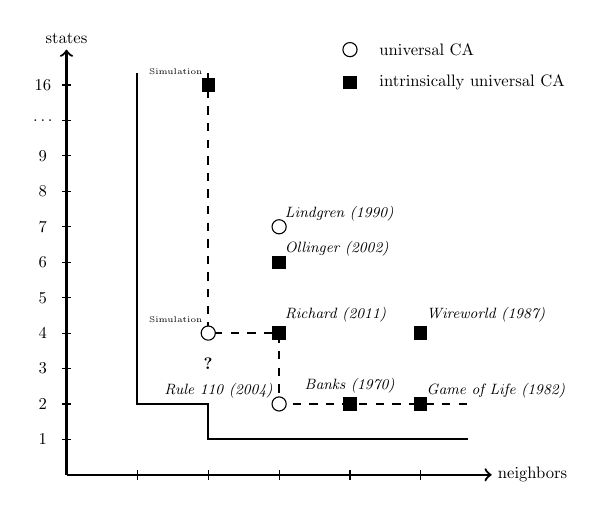
\begin{tikzpicture}[scale=0.6, transform shape]
            % Axes
            \draw[->, thick] (0,0) -- (9,0) node[right] {neighbors};
            \draw[->, thick] (0,0) -- (0,9) node[above] {states};
            
            % Labels
            \node at (1.5,-0.5){
                \radiuszero
            };
            \node at (3,-0.5){
                \oneway
            };
            \node at (4.5,-0.5){
                \radiusone
            };
            \node at (6,-0.5){
                \vonNeumann
            };
            \node at (7.5,-0.5){
                \Moore
            };
            
            \foreach \i in {1,...,5} \draw (1.5*\i,-0.1)--(1.5*\i,0.1);
            \foreach \i in {1,...,9} \node at (-0.5, 0.75*\i){\i};
            \foreach \i in {1,...,11} \draw (-0.1, 0.75*\i)--(0.1, 0.75*\i);
            \node at (-0.5, 0.75*11){16};
            \node at (-0.5, 0.75*10){$\ldots$};
            
            % Universal
            \draw[thick, dashed] (3, 8.5) -- (3, 3) -- (4.5, 3) -- (4.5, 1.5) -- (8.5, 1.5);
            
            % Non-universal
            \draw[thick] (1.5, 8.5) -- (1.5,1.5) -- (3,1.5) -- (3, 0.75) -- (8.5, 0.75);
            
            % universal CA
            \draw[fill=white] (3,3) circle[radius=1.5mm]; % bc
            \node[above left] at (3,3.1) {\tiny{Simulation}};
            \draw[fill=white] (4.5, 5.25) circle[radius=1.5mm]; % bc
            \node[above right] at (4.5,5.25) {\small{\textit{Lindgren (1990)}}};
            \draw[fill=white] (4.5,1.5) circle[radius=1.5mm]; % bc
            \node[above left] at (4.5,1.5) {\small{\textit{Rule 110 (2004)}}};
            \node[] at (3,2.35) {\textbf{?}};
            
            % intrinsically universal CAs
            \filldraw (3, 8.25) node[rectangle, fill=black, minimum size = 1.5mm, inner sep = 4pt] {}; % bc
            \node[above left] at (3,8.35) {\tiny{Simulation}};
            \filldraw (4.5, 4.5) node[rectangle, fill=black, minimum size = 1.5mm, inner sep = 4pt] {}; % bc
            \node[above right] at (4.5,4.5) {\small{\textit{Ollinger (2002)}}};
            \filldraw (4.5, 3) node[rectangle, fill=black, minimum size = 1.5mm, inner sep = 4pt] {}; % bc
            \node[above right] at (4.5,3.1) {\small{\textit{Richard (2011)}}};
            \filldraw (6, 1.5) node[rectangle, fill=black, minimum size = 1.5mm, inner sep = 4pt] {}; % bc
            \node[above] at (6,1.6) {\small{\textit{Banks (1970)}}};
            \filldraw (7.5, 1.5) node[rectangle, fill=black, minimum size = 1.5mm, inner sep = 4pt] {}; % bc
            \node[above right] at (7.5,1.5) {\small{\textit{Game of Life (1982)}}};
            \filldraw (7.5, 3) node[rectangle, fill=black, minimum size = 1.5mm, inner sep = 4pt] {}; % bc
            \node[above right] at (7.5,3.1) {\small{\textit{Wireworld (1987)}}};
            
            
            % Legend
            \begin{scope}[shift={(6,9)}]
                \draw (0,0) circle[fill, radius=1.5mm] {};
                \node[right] at (0.5,0) {universal CA};
            
            
                \draw (0,-0.7) node[rectangle, fill=black, minimum size = 1.5mm, inner sep = 4pt] {};
                \node[right] at (0.5,-0.7) {intrinsically universal CA};
            
            \end{scope}
        \end{tikzpicture}
    \end{subfigure}
    \hspace{0.1em}
    \begin{subfigure}{0.49\textwidth}
        \centering
        \begin{tikzpicture}[scale=0.6, transform shape]
            % background
            \draw[draw=none, pattern=north east lines, pattern color=red] (1.5,8)--(3, 8)--(3, 6)--(1.5, 6)--(1.5, 8);
            \draw[draw=none, pattern=north east lines, pattern color=red] (3,4)--(4.5, 4)--(4.5, 3)--(3, 3)--(3, 4);
            \draw[draw=none, pattern=north east lines, pattern color=red] (-0.5, 2)--(-0.5, 8.5)--(0,8.5)--(0,2)--(-0.5,2);
            
            % Axes
            \draw[->, thick] (-1.5,0) -- (7,0) node[right] {neighbors};
            \draw[->, thick] (-1.5,0) -- (-1.5,9) node[above] {states};
            
            % Labels
            \node at (-0.75,-0.5){
                \radiuszero
            };
            \node at (0,-0.5){
                \oneway
            };
            \node at (1.5,-0.5){
                \radiusone
            };
            \node at (3,-0.5){
                \vonNeumann
            };
            \node at (4.5,-0.5){
                \Moore
            };
            \node at (6,-0.5){
                \innerradiustwo
            };
            \foreach \i in {0,...,4} \draw (1.5*\i,-0.1)--(1.5*\i,0.1);
            \foreach \i in {1,...,8} \node at (-2, \i){\i};
            \foreach \i in {1,...,8} \draw (-1.6, \i)--(-1.4, \i);
            \draw (-0.75,-0.1)--(-0.75,0.1);

            
            
            % Non-universal
            
            \draw[thick] (6.5, 1) -- (0, 1) -- (0, 8);
            \draw[thick] (0, 2) -- (0,1);
            \draw[thick] (0, 2) -- (-0.5,2)--(-0.5, 8.5);
            \draw[thick, color=darkred] (0, 8.5) -- (0,2);
            
            % Universal
            \draw[thick, dashed, color=darkred] (1.5, 8) -- (1.5, 6) -- (3, 6);
            \draw[thick, dashed, color=darkred] (3, 4) -- (3, 3) -- (4.5, 3);
            \draw[thick, dashed] (1.5, 8.5) -- (1.5, 8) --(3, 8) -- (3, 6) -- (3, 5) -- (3, 4) --(4.5, 4) --(4.5, 3) -- (6, 3) -- (6, 2) -- (6.5, 2);
            
            
            % universal ACA
            \draw[fill=white] (1.5,8) circle[radius=1.5mm]; % bc
            \node[above left] at (1.5,8) {\tiny{Simulation}};
            \draw[fill=white] (4.5,3) circle[radius=1.5mm]; % bc
            \node[above right] at (4.5,3) {\small{\textit{Schneider (2012)}}};
            \draw[fill=white] (3, 4) circle[radius=1.5mm]; % bc
            \node[above right] at (3,4) {\small{\textit{Lee (2005)}}};
            \draw[fill=white] (3, 5) circle[radius=1.5mm]; % bc
            \node[above right] at (3,5) {\small{\textit{Lee (2003)}}};
            \draw[fill=white] (6,2) circle[radius=1.5mm]; % bc
            \node[above right] at (6,2) {\small{\textit{Adachi (2010)}}};
            \node[] at (4.5,2) {\textbf{?}};
            \node[] at (3,2) {\textbf{?}};
            \node[] at (1.5,2) {\textbf{?}};
            \node[] at (1.5,3) {\textbf{?}};
            \node[] at (1.5,4) {\textbf{?}};
            \node[] at (1.5,5) {\textbf{?}};
            \filldraw (3, 3) node[rectangle, fill=darkred, minimum size = 1.5mm, inner sep = 4pt] {}; % bc
            \filldraw (1.5, 6) node[rectangle, fill=darkred, minimum size = 1.5mm, inner sep = 4pt] {}; % bc

            
            
            % Legend
            \begin{scope}[shift={(4.5,9)}]
                \draw (0,0) circle[fill, radius=1.5mm] {};
                \node[right] at (0.5,0) {universal ACA};
            
            
                \draw (0,-0.7) node[rectangle, fill=darkred, minimum size = 1.5mm, inner sep = 4pt] {};
                \node[right] at (0.5,-0.7) {improved bounds};
            
            \end{scope}
        \end{tikzpicture}
    \end{subfigure}
    \caption{Current ``universality frontier'' for synchronous (left) and asynchronous cellular automata (right). The solid line indicates the impossibility proofs for universality, while the dashed line shows the currently smallest known universal constructions. Contributions of this work are marked in red: $6$-state first neighbors, $3$-state von Neumann, and non-universality of one-way automata.}
    \label{fig:asynchronous-frontier}
\end{figure}

\subparagraph*{Our contributions} We present a comprehensive overview of computational abilities of (a)synchronous cellular automata and propose a formal definition for the notion of simulation with ACAs, which, although often used implicitly, has been missing in the literature \cite{nakamura, improved-soldiers, worsch-intrinsically, golze}. We adopt the ``adversarial'' view on asynchrony, i.e. require the ACAs to be robust against \emph{any} asynchronous updating (other notions such as randomized and ``best-case'' asynchrony have also been studied \cite{aca-survey}). By combining various simulation techniques and known universality constructions, we assemble an explicit ``universality frontier'' for CAs and ACAs, i.e., the boundary between universal and non-universal computation, similarly to how it was already done for Turing machines \cite{small-utms} (see Figure \ref{fig:asynchronous-frontier}). The dashed line represents the best-known upper bound on universality constructions, while the filled line represents the best-known lower bound for non-universality constructions. We further present our own contributions to both asynchronous simulation and the ``universality frontier'':
%
\begin{itemize}
    \item In \cref{sec:flip-automata-networks}, we introduce a simple asynchronous model of computation---the flip automata network (FAN), which computation stays invariant in any asynchronous setting.
    \item In \cref{sec:simulation} we show that by using FANs as a middleman, ACAs can simulate their synchronous counterparts with just $4q$ states (and $3q$ in the $1$-dimensional case), improving on the previous constructions which had quadratic overhead.
    \item In \cref{sec:non-universal} we extend the ``universality frontier'' by deriving a non-universality result for one-way asynchronous automata, demonstrating their computational equivalence to classical finite-state machines. This hints that bidirectional communication is crucial for achieving universality in ACAs (which is not the case for classical CAs).
    \item In \cref{sec:small-aca} we present smaller universal ACAs than previously known: a universal $3$-state von Neumann automaton and a universal $6$-state first-neighbors automaton.
\end{itemize}
%
\section{Background}\label{sec:background}

\begin{definition}[Cellular Automaton]\label{def:cellular-automaton}
    A $d$-dimensional cellular automaton (CA) is a tuple $(S, N, f, \mathbb{Z}^d)$ where $f: S^k \rightarrow S$ is the local rule function, $S$ is the set of \emph{states}, $N = (n_1, n_2, \ldots, n_k)$ is the neighborhood vector (defines relative neighbors for each cell) and $\mathbb{Z}^d$ is the cellular space.
\end{definition}
%
We call a neighborhood $N$ \emph{symmetric} if $-1 \cdot N$ is a permutation of $N$, and two cells are \emph{neighboring} if they are both in the neighborhoods of each other. While there are infinitely many choices for the neighborhood vector $N$, there are four types of neighborhoods that are considered canonical and have been researched the most (note that both Moore and von Neumann generalize naturally to arbitrary dimension $d$, and first-neighbors is the $1$-dimensional case for both of them):
\begin{center}
    \emph{One-way}\raisebox{-3pt}{\oneway} \quad \emph{First neighbors}\raisebox{-3pt}{\radiusone} \quad \emph{Von Neumann}\raisebox{-6pt}{\vonNeumann} \quad \emph{Moore}\raisebox{-6pt}{\Moore}
\end{center}

A \emph{configuration} of a $d$-dimensional cellular automaton is a function $c: \Z^d \longrightarrow S$, which assigns a state to every cell in the cellular space. At each timestamp $t$, every cell $i \in \Z^d$ synchronously applies the local rule function to its local neighborhood $N$, causing the complete configuration to transition to a new configuration $c_{t+1}$. For each cell $i$ the next state $c_{t+1}(i)$ is defined as
%
\begin{equation*}
    c_{t+1}(i) = f(c_t(i + n_0), \ldots, c_t(i + n_k))
\end{equation*}

We can characterize the transformation between two consecutive configurations of a cellular automaton by specifying the \emph{global transition function} $G: S^{\Z^d} \longrightarrow S^{\Z^d}$ with $G(c_k) = c_{k+1}$. 

\begin{definition}[Asynchronous Cellular Automaton]\label{def:aca}
    An asynchronous cellular automaton $\mathbb{A} = (S, N, f, \mathbb{Z}^d)$ is a cellular automaton that chooses at each point in time $t$ an update set $D_t \subseteq \Z^d$ and applies the local rule function $f$ only to cells in $D_t$.
\end{definition}

Definition \ref{def:aca} presents the most common type of asynchronous updating, also referred to as \emph{purely} asynchronous. Other notions such as \emph{$\alpha$-asynchrony} (each cell updates independently with probability $\alpha$) have been also considered, for a comprehensive survey we refer to Fatès \cite{aca-survey}. 

\begin{definition}[Update Schedule]
    For an asynchronous cellular automaton $\mathbb{A} = (S, N, f, \Z^d)$ we define the asynchronous update schedule $\zeta : \N \longrightarrow \PS{\Z^d}$ a function specifying the subsets of cells updated at each point $t$ in time. $\zeta$ is required to have the property that every $i \in S^{\Z^d}$ appears infinitely often in $\Ima{\zeta}$, or, in other words, every cell is updated infinitely often.
\end{definition}

In the case of a purely asynchronous setting $\zeta$ can be arbitrary: we can imagine an ``adversary'' that can choose any schedule to update $\mathbb{A}$. Given an update schedule $\zeta$ we can identify the global asynchronous transition function $G^\zeta$ and the corresponding \emph{asynchronous space-time} $\spacetime^\zeta \colon \N \times \Z^d \longrightarrow S$ which maps configurations to their evolved asynchronous counterparts, i.e. $\spacetime^\zeta(0, c_0) = c_0$ and $\spacetime^\zeta(t, c_0) = c_t^\zeta$ such that
%
\begin{equation*}
    c^\zeta_{t+1} = G^\zeta(c_t) = G_{\zeta(t)}(c_t) \quad \text{where} \quad G_D(c)(i) = 
    \left\{ \begin{array}{rc} 
    G(c)(i) & \mbox{if} \quad i \in D \\ 
    c(i) & \mbox{otherwise} 
    \end{array}\right.
\end{equation*}
%
Furthermore, we call a cell $i \in \mathbb{Z}^d$ \emph{active} (on configuration $c$) if and only if $G(c)(i) \neq c(i)$.
%
\begin{definition}[Update History]
    Given an asynchronous cellular automaton $\mathbb{A}$ under same update schedule $\zeta$, we define the update history as a sequence of configurations $h_0, h_1, \ldots$ where $h_0 = c_0$ and $h_t(i) = c_{t'_i}(i)$ with
    \begin{equation*}
         t'_i = \min \{a_t \in \N \ | \ \exists a_0 \ldots a_{t-1} \ \forall j < t \ (a_j < a_{j+1} \wedge c_{a_j}(i) \neq c_{a_{j+1}}(i)) \}
    \end{equation*} 
    if such $t'_i$ exists, and undefined otherwise.
\end{definition}

Intuitively, the update history records the asynchronous space-time ``up to value equality'' where for each cell $i$ we only record ``true'' updates to the value of $i$, discarding the information about the updates that did not change the value and the specific time when these updates occurred (in particular, the history can also be finite!). We say that an ACA $\mathbb{A}$ has \emph{invariant histories on configuration $c_0$} if any update schedule of $\mathbb{A}$ initialized with $c_0$ results in the same update history. Similarly, we say that $\mathbb{A}$ has \emph{invariant histories} if it has invariant histories for any initial configuration. Such ACAs form a particularly important subclass of cellular automata, since they allow for reliable computations without any need for global synchronization. 

Gács \cite{gacs} has given an almost complete characterization of ACAs with invariant histories using just algebraic properties of monotonicity and commutativity.

\begin{definition}[Monotonicity]
    A global transition function $G$ is \textit{monotonic} if for any configuration $c$, active cell $i$ and an update set $A \subseteq \mathbb{Z}^d \setminus \{i\}$ it holds that
    \begin{equation*}
        G_{\{i\}}(G_A(c))(i) \neq c(i)
    \end{equation*}
\end{definition}

In other words, an update of any other cell cannot prohibit the cell $i$ from updating itself, essentially ensuring a sort of ``lock-free'' computation flow.

\begin{definition}[Commutativity]\label{def:commutativity}
    A global transition function $G$ is \textit{commutative} if for any configuration $c$ and two disjoint update sets of active cells $A, B \subseteq \mathbb{Z}^d$ it holds
    \begin{equation*}
        G_A(G_B(c)) = G_{A \cup B}(c) = G_B(G_A(c))
    \end{equation*}
\end{definition}

Effectively, this implies that the updates of simultaneously active cells can be performed in any order. We say that the cellular automaton is \emph{commutative} if its global transition function is commutative. 
%
\begin{theorem}[Invariance \cite{gacs}]\label{thm:commutativity}
    A cellular automaton $(S, N, f, \mathbb{Z}^d)$ is commutative if and only if it has invariant histories and the its global transition function $G$ is monotonic.
\end{theorem}

Even though commutativity does not characterize all automata with invariant histories (this question was shown to be undecidable in the same paper), it characterizes a very natural subclass thereof, since monotonicity is in general a desirable property to have. Furthermore, commutativity can be verified algorithmically---due to the local structure of $G$ it is in fact sufficient to check the conditions in \cref{def:commutativity} only for cases where $A$ and $B$ are singleton update sets, i.e. whether $G_{\{i\}}(G_{\{j\}}(c)) = G_{\{i, j\}}(c)$ holds for any cells $i, j \in \mathbb{Z}^d$. A more in-depth explanation is given in \cref{example:local-commutativity}.

A generalization of commutativity for automata networks---an extension of cellular automata allowing arbitrary spaces and nonuniform local rule functions---is known, but requires more complex machinery \cite{automata-networks}. We note that while the algebraic characterization provides a simple way of verifying for invariant histories in ACAs, it is generally hard to design commutative ACAs with desired properties without inducing a large state complexity overhead. These issues arise due to the lack of a general ``constructive'' understanding of such ACAs, something that we attempt to mitigate in the sections below. 

\section{Flip Automata Networks}\label{sec:flip-automata-networks}

In this section, we present a simple asynchronous distributed model of computation called flip automata networks (FAN). While FANs are just a simple modification of automata networks, they have the advantage of having invariant histories by design, allowing us to build a simple bridge between CAs and ACAs.

\begin{definition}[Flip Automata Network]
    A \emph{flip automata network} $\mathcal{A}_\text{flip}$ is a triple $(T, S, {\{f_i\}}_{i\in I})$ where $T = (I, E)$ is a undirected graph with edges $E \subseteq \{ \{v_i, v_j \} \ | \ i \neq j \wedge v_i, v_j \in I \}$ such that each edge has a direction indicator $\in {\{ \nearrow, \swarrow \}}$, neighborhood function
    \begin{equation*}
        N(v_i) = \{ v \in I \ | \ \{v, v_i\} \in E \} 
    \end{equation*} 
    which has to be finite for all $v_i \in I$, $S$ is a state set and ${\{f_i\}}_{i \in I}$ is the set of all flip functions where
    \begin{equation*}
        f_i: S^{N(v_i) \cup \{v_i\}} \longrightarrow S \times {\{ \nearrow, \swarrow \}}^{N(v_i)}
    \end{equation*}
    is the flip function associated with vertex $v_i$ ($\nearrow$ ``points'' to the node with the larger index and $\swarrow$ to the node with the smaller index). A function $f_i$ is only applicable if the direction indicator on all edges between $N(v_i)$ and $v_i$ ``point'' towards $v_i$, and the application of $f_i$ can update the state of $v_i$ and ``flip'' the direction indicator on any of the edges from $N(v_i)$. 
\end{definition}

Similarly to classical automata networks, individual transition functions can be applied in some (arbitrary) order. Flip automata networks have an intuitive interpretation: the arrows indicate directed information sharing and every node waits for all of its neighbors to share before preforming a transition, as shown in Figure \ref{fig:causal-network}.

\begin{figure}[H]
    \centering
    \begin{tikzpicture}[
            > = stealth, % arrow head style
            shorten > = 1pt, % don't touch arrow head to node
            auto,
            node distance = 2cm, % distance between nodes
            semithick, % line style,
            scale=0.75, transform shape
        ]
        \tikzstyle{every state}=[
            draw = black,
            thick,
            fill = white,
            minimum size = 4mm
        ]
        \node[state, fill=lightgray!30] (s) {$1$};
        \node[state] (s1) [above right=0.7cm and 0.7cm of s] {$1$};
        \node[state] (s2) [below right=0.7cm and 0.7cm of s] {$1$};
        \node[state] (s3) [above left=0.7cm and 0.7cm of s] {$1$};
        \node[state] (s4) [below left = 0.7cm and 0.7cm of s] {$1$};

        \path[->] (s1) edge node{} (s);
        \path[->] (s2) edge node{} (s);
        \path[->] (s3) edge node{} (s);
        \path[->] (s4) edge node{} (s);
        \path[->] (s2) edge node{} (s1);
        \path[->] (s3) edge node{} (s1);
        \path[->] (s2) edge node{} (s4);
        \path[->] (s3) edge node{} (s4);
    \end{tikzpicture}
    %
    \hspace{3em}
    %
    \begin{tikzpicture}[
            > = stealth, % arrow head style
            shorten > = 1pt, % don't touch arrow head to node
            auto,
            node distance = 2cm, % distance between nodes
            semithick, % line style,
            scale=0.75, transform shape
        ]

        \tikzstyle{every state}=[
            draw = black,
            thick,
            fill = white,
            minimum size = 4mm
        ]

        \node[state] (s) {$2$};
        \node[state, fill=lightgray!30] (s1) [above right=0.7cm and 0.7cm of s] {$1$};
        \node[state] (s2) [below right=0.7cm and 0.7cm of s] {$1$};
        \node[state] (s3) [above left=0.7cm and 0.7cm of s] {$1$};
        \node[state, fill=lightgray!30] (s4) [below left = 0.7cm and 0.7cm of s] {$1$};

        \path[->] (s) edge node{}  (s1);
        \path[->] (s) edge node{} (s2);
        \path[->] (s) edge node{} (s3);
        \path[->] (s) edge node{} (s4);
        \path[->] (s2) edge node{} (s1);
        \path[->] (s3) edge node{} (s1);
        \path[->] (s2) edge node{} (s4);
        \path[->] (s3) edge node{} (s4);

    \end{tikzpicture}
    %
    \hspace{3em}
    %
    \begin{tikzpicture}[
            > = stealth, % arrow head style
            shorten > = 1pt, % don't touch arrow head to node
            auto,
            node distance = 2cm, % distance between nodes
            semithick, % line style
            scale=0.75, transform shape
        ]

        \tikzstyle{every state}=[
            draw = black,
            thick,
            fill = white,
            minimum size = 4mm
        ]

        \node[state] (s) {$2$};
        \node[state] (s1) [above right=0.7cm and 0.7cm of s] {$2$};
        \node[state, fill=lightgray!30] (s2) [below right=0.7cm and 0.7cm of s] {$1$};
        \node[state, fill=lightgray!30] (s3) [above left=0.7cm and 0.7cm of s] {$1$};
        \node[state] (s4) [below left = 0.7cm and 0.7cm of s] {$2$};

        \path[->] (s1) edge node{}  (s);
        \path[->] (s) edge node{} (s2);
        \path[->] (s) edge node{} (s3);
        \path[->] (s4) edge node{} (s);
        \path[->] (s1) edge node{} (s2);
        \path[->] (s1) edge node{} (s3);
        \path[->] (s4) edge node{} (s2);
        \path[->] (s4) edge node{} (s3);
    \end{tikzpicture}
    \caption{Two-step evolution of flip automata network $\mathcal{A}_\text{flip} = (T_{\text{flip}}, \{0, 1, 2\}, \{f_i\}_{i=0}^4)$ where each $f_i$ computes the sum of all neighboring node states mod $3$, and flips all incoming arrows. At each point in time only gray colored nodes have applicable flip function.}
    \label{fig:causal-network}
\end{figure}

\begin{restatable}{proposition}{fliptheorem}\label{prop:flip-invariant}
    Flip automata networks have invariant histories, i.e., the update schedule does not affect the update history of individual nodes.
\end{restatable}

The proof for Proposition \ref{prop:flip-invariant} can be found in Appendix \ref{sec:ommited-proof}. In the following sections, we will show that flip automata networks can be embedded into asynchronous cellular automata with minimal overhead, allowing for simpler simulation techniques and smaller universality constructions. A simple embedding is given in Example \ref{ex:mountain-valley} below.

\begin{example}\label{ex:mountain-valley}
    Consider an asynchronous version of \rle{212}. The only transitions that affect the cell state are $(100) \mapsto 1$ and $(011) \mapsto 0$, in all other cases the cell does not change its state. Observe that no two neighboring cells can be active at the same time. Using the local neighborhood of each cell, we can interpret \rle{212} as a $1$-dimensional flip automata network. To this end we define a mapping $\psi$ that adds directional indicators between adjacent cells $i$ and $i+1$ based on their current states in some configuration $c$:
    \begin{align*}
        &\psi(c(i), c(i+1)) = c(i) \longleftarrow c(i+1) \quad \text{for $c(i) = c(i+1)$}\\
        &\psi(c(i), c(i+1)) = c(i) \longrightarrow c(i+1) \quad \text{for $c(i) \neq c(i+1)$}
    \end{align*}
    This allows us to transform any configuration of \rle{212} into a configuration of a flip automata network. For example, the following synchronous update of configuration $c$
    \begin{center}
        $\ldots 100110011 \ldots \mapsto \ldots 110011001 \ldots$
    \end{center}
    can be seen as an update in the flip automata network where all applicable transitions flip:
    \begin{center}
        $\fbox{1} \longrightarrow \fbox{0} \longleftarrow \fbox{0} \longrightarrow \fbox{1} \longleftarrow \fbox{1} \longrightarrow \fbox{0} \longleftarrow \fbox{0} \longrightarrow \fbox{1} \longleftarrow \fbox{1}$ \\
        $\Downarrow$\\
        $\fbox{1} \longleftarrow \fbox{1} \longrightarrow \fbox{0} \longleftarrow \fbox{0} \longrightarrow \fbox{1} \longleftarrow \fbox{1} \longrightarrow \fbox{0} \longleftarrow \fbox{0} \longrightarrow \fbox{1}$
    \end{center}
    %
    Furthermore, if we think of $\longrightarrow$ as $\diagdown$ slope and of $\longleftarrow$ as $\diagup$ slope we can visualize any configuration of such flip automata network as a zigzag line in a $2$-dimensional space, which we will refer to as a \emph{mountain-valley} landscape, as shown in Figure \ref{fig:wave} (left). The update history of configuration $c$ under some asynchronous update schedule can thus be visualized as a $2$-dimensional ``fluid'' slowly filling the space-time $\mathbb{Z} \times t$, where at each point in time some subset of ``valleys'' become ``mountains''. Depending on the update schedule $\zeta$ some mountains will grow faster than others, however since every cell will be updated infinitely often, the ``fluid'' is guaranteed to fill the full space-time, as sketched in Figure \ref{fig:wave} (right). 
    %
    \begin{figure}[t]
    \centering
    \begin{subfigure}{0.475\textwidth}
        \centering
        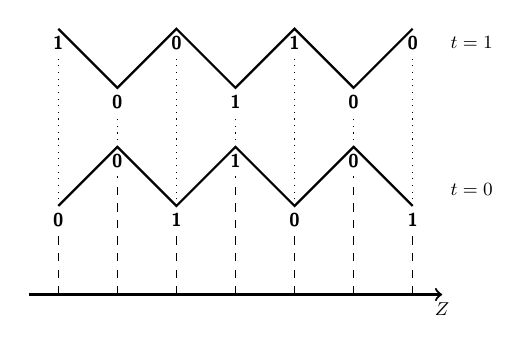
\begin{tikzpicture}[font=\sffamily\small, scale=0.75, transform shape]
        
        \draw[->, thick] (-0.5,0.5) -- (6.5,0.5) node[below] {$\mathbb{Z}$};
        
        
        \draw[black, thick] (0,2) -- (1, 3) -- (2, 2) -- (3, 3) -- (4, 2) -- (5, 3) -- (6, 2);
        \draw[black, thick] (0,5) -- (1, 4) -- (2, 5) -- (3, 4) -- (4, 5) -- (5, 4) -- (6, 5);

        \draw[dotted] (0, 2) -- (0, 4.5);
        \draw[dotted] (1, 3) -- (1, 3.5);
        \draw[dotted] (2, 2) -- (2, 4.5);
        \draw[dotted] (3, 3) -- (3, 3.5);
        \draw[dotted] (4, 2) -- (4, 4.5);
        \draw[dotted] (5, 3) -- (5, 3.5);
        \draw[dotted] (6, 2) -- (6, 4.5);

        \draw[dashed] (0, 0.5) -- (0, 1.5);
        \draw[dashed] (1, 0.5) -- (1, 2.5);
        \draw[dashed] (2, 0.5) -- (2, 1.5);
        \draw[dashed] (3, 0.5) -- (3, 2.5);
        \draw[dashed] (4, 0.5) -- (4, 1.5);
        \draw[dashed] (5, 0.5) -- (5, 2.5);
        \draw[dashed] (6, 0.5) -- (6, 1.5);
        
        \node[below] at (0,2) {\textbf{0}};
        \node[below] at (2,2) {\textbf{1}};
        \node[below] at (4,2) {\textbf{0}};
        \node[below] at (6,2) {\textbf{1}};
        
        \node[below] at (1,3) {\textbf{0}};
        \node[below] at (3,3) {\textbf{1}};
        \node[below] at (5,3) {\textbf{0}};
        \node[below] at (7,2.5) {$t = 0$};
        
        
        \node[below] at (0,5) {\textbf{1}};
        \node[below] at (2,5) {\textbf{0}};
        \node[below] at (4,5) {\textbf{1}};
        \node[below] at (6,5) {\textbf{0}};
        
        \node[below] at (1,4) {\textbf{0}};
        \node[below] at (3,4) {\textbf{1}};
        \node[below] at (5,4) {\textbf{0}};
        \node[below] at (7,5) {$t = 1$};
        
        \end{tikzpicture}
    \end{subfigure}
    \begin{subfigure}{0.475\textwidth}
        \centering
        \begin{tikzpicture}[font=\sffamily\small, scale=0.75, transform shape]]
        \draw[->, thick] (1.0,1.0) -- (8,1.0) node[below] {$\mathbb{Z}$};
        \draw[->, thick] (1.0,1.0) -- (1.0,5.5) node[left] {$t$};
        
        
        \draw[thick, pattern=horizontal lines light gray] (1,1.0) -- (1, 3.5) -- (1.5, 3) -- (2, 3.5) -- (2.5, 4) -- (3, 3.5) -- (4, 4.5) -- (4.5, 5) -- (5, 4.5) -- (6, 3.5) -- (6.5, 4) -- (7, 3.5) --(7.5, 3) -- (7.5, 1.0) -- cycle;
        
        \draw[dashed] (1, 1.0) -- (1, 3.5);
        \draw[dashed] (1.5, 1.0) -- (1.5, 3);
        \draw[dashed] (2, 1.0) -- (2, 3.5);
        \draw[dashed] (2.5, 1.0) -- (2.5, 4);
        \draw[dashed] (3, 1.0) -- (3, 3.5);
        \draw[dashed] (3.5, 1.0) -- (3.5, 4);
        \draw[dashed] (4, 1.0) -- (4, 4.5);
        \draw[dashed] (4.5, 1.0) -- (4.5, 5);
        \draw[dashed] (5, 1.0) -- (5, 4.5);
        \draw[dashed] (5.5, 1.0) -- (5.5, 4);
        \draw[dashed] (6, 1.0) -- (6, 3.5);
        \draw[dashed] (6.5, 1.0) -- (6.5, 4);
        \draw[dashed] (7, 1.0) -- (7, 3.5);
        
        \draw[dotted, semithick] (1, 3.5) -- (1.5, 4)--(2, 3.5);
        \draw[dotted, semithick] (2.5, 4) -- (3, 4.5)--(3.5, 4);
        \draw[dotted, semithick] (5.5, 4) -- (6, 4.5)--(6.5, 4);
        
        \draw[thick, >=stealth, ->] (1.5, 3) -- (1.5, 4);
        \draw[thick, >=stealth, ->] (3, 3.5) -- (3, 4.5);
        \draw[thick, >=stealth, ->] (6, 3.5) -- (6, 4.5);
        
        \end{tikzpicture}
    \end{subfigure}
    \caption{Representation of a flip automata network for \rle{212} as a mountain-valley landscape (left) and evolution of a mountain-valley landscape carrying information about the frequency of updates (right).}
    \label{fig:wave}
    \end{figure}

\end{example}

\begin{restatable}{lemma}{causality}\label{lem:causality}
    Every ACA $\mathbb{A} = (S, N, f, \mathbb{Z}^d)$ with von Neumann neighborhood where no two neighboring cells can be active at the same time corresponds precisely to a FAN $\mathcal{A}$ with the same state set $S$, and the topology of $\mathcal{A}$ has a bijection to the cells of $\mathbb{A}$.
\end{restatable}

The proof for this result is similar to Example \ref{ex:mountain-valley} and can be found in Appendix \ref{sec:ommited-proof}, and as a direct consequence we obtain that all such ACAs have invariant histories due to \cref{prop:flip-invariant} (this invariance can be alternatively proven using commutativity). Lemma \ref{lem:causality} demonstrates the duality between a large subclass of ACAs and FANs, which will prove useful in understanding the computational mechanics of asynchronous automata.

\begin{openquestion}
    Does there exist a constructive characterization for all commutative cellular automata using FANs (or a minor modification thereof)?
\end{openquestion}

\section{Simulating Synchronous Networks}\label{sec:simulation}

We start by discussing the notion of simulation between cellular automata and present its extension to the asynchronous scenario. For brevity, we refer to the simulated (synchronous) automaton as the ``guest'' CA, and the simulating (a)synchronous automaton as the ``host''.

\begin{definition}[Direct Simulation]
    A cellular automaton $B = (S^B, N^B, f^B, \mathbb{Z}^d)$ with global function $G^B$ \emph{directly simulates} a cellular automaton $A = (S^A, N^A, f^A, \mathbb{Z}^d)$ with global function $G^A$ of the same dimension according to a mapping $\psi: S^A \longrightarrow \mathcal{P}(S^B)$ if for all states $a, b \in S^A$ we have $\psi(a) \cap \psi(b) = \varnothing$ and for any configuration $c \in {(S^A)}^{\Z^d}$ we have 
    \begin{equation*}
        \{ G^B(c') \ | \ c' \in \psi(c) \} \subseteq \psi(G^A(c))
    \end{equation*}
    i.e. all encodings $c'$ evolve in $B$ as $c$ evolves in $A$, in which case we write $G^A \prec G^B$.
\end{definition}

The general definition of simulation extends the definition of direct simulation by allowing packing, cutting, and shifting, such that a direct simulation can occur.

\begin{definition}[Unpacking Map]\label{def:direct-simulation}
    Let $S$ be a state set and $m = (m_1, \ldots, m_d)$ be a tuple of positive integers, then the unpacking bijective map
    \begin{equation*}
        o_m: {\big(S^{\prod m_i}\big)}^{\Z^d} \longrightarrow S^{\Z^d}
    \end{equation*}
    is defined for any configuration $c \in {\big(S^{\prod m_i}\big)}^{\Z^d}$ such that for any position $i \in \Z^d$ and offset $r \in \prod_i \Z_{m_i}$ it holds that $o_m(c)(m_1i_1 + r_1, \ldots, m_d i_d + r_d) = c(i)(r)$. 
\end{definition}

In essence, the unpacking map $o_m$ transforms every cell $i$ with state from $S^{\prod m_i}$ into a block of cells of size $\prod m_i$ and bijectively maps the state information from $i$ to the block. We will refer to the scalar $|m|$ as the \emph{sparsity} of the unpacking.

\begin{definition}[Simulation \cite{Ollinger-chapter}]\label{def:simulation}
    A cellular automaton $B = (S^B, N^B, f^B, \mathbb{Z}^d)$ simulates a  cellular automaton $A = (S^A, N^A, f^A, \mathbb{Z}^d)$ if there exists an unpacking map $o_m$, a translation $\tau_v$ and a positive integer $n \in \N$ such that
    \begin{equation*}
        G^A \prec o_m^{-1} \circ {(G^B)}^n \circ o_m \circ \tau_v
    \end{equation*}
    In this case, we say that $B$ simulates $A$ in $n$-linear time (and in real time if $n = 1$).
\end{definition}

For the asynchronous scenario multiple simulation definitions have been proposed, however, all of them have turned out to be either too restrictive or flawed \cite{nakamura, improved-soldiers}. Most notably, they did not support for ``transitivity'', i.e., if an asynchronous automaton $\mathbb{C}$ simulates synchronous automaton $B$, and $B$ in turn simulates another synchronous automaton $A$, then one would expect $\mathbb{C}$ to simulate $A$ (which was not fulfilled). To mitigate these issues, we propose a natural extension of Definition \ref{def:simulation} based on the notion of synchronous simulation and invariant histories, such that it is general enough to encompass all of the previous simulation constructions, while preserving the crucial property of ``transitivity''.

\begin{definition}[Invariant Simulation]\label{def:invariant}
     Let $\mathbb{B} = (S^B, N^B, f^B, \mathbb{Z}^d)$ be an ACA and $A = (S^A, N^A, f^A, \mathbb{Z}^d)$ be some synchronous CA of the same dimension, and let
     \begin{equation*}
         H^B: {(S^B)}^{\Z^d} \longrightarrow {(S^B)}^{\Z^d}
     \end{equation*}
     be a function that transforms the configuration by mapping every cell $i$ in state $h_t(i)$ to the next point in its invariant update history $h_{t+1}(i)$ under $\mathbb{B}$. In case $\mathbb{B}$ does not have invariant histories for some configuration $c$, then $H^B(c)$ is undefined. We say that $\mathbb{B}$ invariantly simulates $A$ if there exists an unpacking map $o_m$, a translation $\tau_v$ and a positive integer $n \in \N$ such that 
     \begin{equation*}
        G^A \prec o_m^{-1} \circ {(H^B)}^n \circ o_m \circ \tau_v
    \end{equation*}
    where $n$ is again the linear time parameter.
\end{definition}

\cref{def:invariant} requires configurations of $A$ to appear as complete, encoded rows in the invariant history $h$ of $\mathbb{B}$, allowing the observer to reconstruct the evolution of $A$ from the evolution of $\mathbb{B}$, even if the update schedule $\zeta$ is unknown. The ``transitivity'' is trivially fulfilled, since we can chain the unpackings and translations between different types fo simulation.

\subparagraph*{Simulation techniques} The classical approach to asynchronous simulation requires the ``host'' ACA to be of the same dimension $d$ and neighborhood $N$ as the ``guest'' CA---the rationale is that the underlying machine can no longer be ran synchronously. The classical   $3q^2$ real time construction by Nakamura \cite{nakamura, gacs} and $q^2 + 2q$ state $3$-linear time construction in \cite{improved-soldiers, worsch-intrinsically} achieve this by increasing the number of states in the ``host'' (given a $q$-state ``guest'' CA). Furthermore, the simulations require the neighborhood $N$ to be symmetric (this constraint will be investigated more in \cref{sec:universality}). Our new construction---based on embedding of flip automata networks into ACAs---allows for simulations with both linear state and time overheads. We restrict the neighborhood $N$ to be either von Neumann or Moore, since these constitute the most crucial cases.

\begin{proposition}[Mountain-Valley Encoding]\label{prop:mountain-valley}
    For a synchronous automaton $A = (S, N, f, \Z^d)$ with von Neumann or Moore neighborhood $N$ we can construct an asynchronous cellular automaton $\mathbb{B} = (S \times \{0, 1, 2, 3\}, N, f', \Z^d)$ which simulates $A$ in real time.
\end{proposition}

\begin{proof}
    The high-level idea behind the construction of $\mathbb{B}$ is that we first construct a flip automata network $\mathcal{A}$ which simulates $A$, and then create an asynchronous cellular automaton embedding $\mathcal{A}$. To keep the construction elegant, we present it for the $2$-dimensional von Neumann neighborhood $N = ((-1, 0), (1, 0), (0, 0), (0, 1), (0, -1))$ in detail, and give a sketch for Moore's neighborhood. The generalization to any dimension $d$ is straightforward.
    
    Consider a FAN $\mathcal{A} = (T = \Z^2, S, \{f_\textbf{E}, f_\textbf{O}\})$ with the same set of states as $A$, where we distinguish between two types of nodes \textbf{E} and \textbf{O}, and set $\oplus / \ominus$ to be addition and subtraction mod $|S|$. Then, for von Neumann neighborhood:
    \begin{itemize}
        \item \textbf{E} nodes are placed on coordinates $(2i, 2j) \in \Z^2$ and we set
        %
        \begin{equation*}
            f_\textbf{E}(s_{(1, 0)}, s_{(0, 1)}, s, s_{(-1, 0)}, s_{(0, -1)}) = f(s_{(1, 0)} \ominus s, s_{(0, 1)} \ominus s, s, s_{(-1, 0)} \ominus s, s_{(0, -1)} \ominus s)
        \end{equation*}
        %
        Intuitively, \textbf{E} nodes store the states of the cells in $A$ and simulate the local transition $f$
        \item \textbf{O} nodes are placed at all remaining coordinates and every $f_\textbf{O}$ computes the sum $\oplus$ of all of its \textbf{E} neighbors. On a high level, \textbf{O} nodes use \textsf{XOR} to accumulate and pass on the information about (simulated) neighbors of \textbf{E}
    \end{itemize}
    Observe the topology of $\mathcal{A}$ as it is presented in Figure \ref{fig:mountain-valley}---the directional indicators are only added between neighboring \textbf{E} and \textbf{O} nodes. For von Neumann neighborhood (left) the \textbf{O} nodes with odd coordinates will be isolated in $\mathcal{A}$ since they do not have any \textbf{E} neighbors. On the other hand, in the case of Moore's neighborhood (right), the topology of $\mathcal{A}$ becomes non-uniform with different \textbf{O} nodes having different neighborhoods. We initialize $\mathcal{A}$ with all directional indicators pointing from \textbf{E} nodes to \textbf{O} nodes, and on every local transition we flip all edges. Furthermore, the initial configuration $c_0$ of $A$ is encoded on the \textbf{E} nodes, where $T(2i) = c_0(i)$, and \textbf{O} nodes are initialized arbitrarily. If we first update all \textbf{O} nodes, flip the arrows, and update all \textbf{E} nodes, the state of the network will be an encoding of $G^A(c_0)$.
    %
    \begin{figure}[tb]
    \centering
    \begin{tikzpicture}[font=\sffamily\small, scale=0.7, transform shape]
    \draw[->, thick] (0.0,0.0) -- (4.0,0.0) node[below] {$\Z$};
    \draw[->, thick] (0.0,0.0) -- (0.0,4.0) node[left] {$\Z$};

    \foreach \i in {0,...,5}{
        \draw[dashed] (0.75*\i, 0) -- (0.75*\i, 3.75);
        \draw[dashed] (0, 0.75*\i) -- (3.75, 0.75*\i);
    }

    \foreach \i in {0,...,2}{
        \draw[<-, color=darkred, thick, >=stealth] (0.375 + 1.5*\i, 0.6) -- (0.375 + 1.5*\i, 0.9);
        \draw[<-, color=darkred, thick, >=stealth] (0.375 + 1.5*\i, 2.1) -- (0.375 + 1.5*\i, 2.4);
        \draw[->, color=darkred, thick, >=stealth] (0.375 + 1.5*\i, 1.35) -- (0.375 + 1.5*\i, 1.65);
        \draw[->, color=darkred, thick, >=stealth] (0.375 + 1.5*\i, 2.85) -- (0.375 + 1.5*\i, 3.15);
    }  

    \foreach \i in {0,...,2}{
        \draw[<-, color=darkred, thick, >=stealth] (0.6, 0.375 + 1.5*\i) -- (0.9, 0.375 + 1.5*\i);
        \draw[<-, color=darkred, thick, >=stealth] (2.1, 0.375 + 1.5*\i) -- (2.4, 0.375 + 1.5*\i);
        \draw[->, color=darkred, thick, >=stealth] (1.35, 0.375 + 1.5*\i) -- (1.65, 0.375 + 1.5*\i);
        \draw[->, color=darkred, thick, >=stealth] (2.85, 0.375 + 1.5*\i) -- (3.15, 0.375 + 1.5*\i);
    }

    \node[] at (0.375,0.375) {$\textbf{E}$};
    \node[] at (1.125,0.375) {$\textbf{O}$};
    \node[] at (1.875,0.375) {$\textbf{E}$};
    \node[] at (2.625,0.375) {$\textbf{O}$};
    \node[] at (3.375,0.375) {$\textbf{E}$};

    \node[] at (0.375,1.125) {$\textbf{O}$};
    \node[] at (1.125,1.125) {$\textbf{O}$};
    \node[] at (1.875,1.125) {$\textbf{O}$};
    \node[] at (2.625,1.125) {$\textbf{O}$};
    \node[] at (3.375,1.125) {$\textbf{O}$};

    \node[] at (0.375,1.875) {$\textbf{E}$};
    \node[] at (1.125,1.875) {$\textbf{O}$};
    \node[] at (1.875,1.875) {$\textbf{E}$};
    \node[] at (2.625,1.875) {$\textbf{O}$};
    \node[] at (3.375,1.875) {$\textbf{E}$};

    \node[] at (0.375,2.625) {$\textbf{O}$};
    \node[] at (1.125,2.625) {$\textbf{O}$};
    \node[] at (1.875,2.625) {$\textbf{O}$};
    \node[] at (2.625,2.625) {$\textbf{O}$};
    \node[] at (3.375,2.625) {$\textbf{O}$};

    \node[] at (0.375,3.375) {$\textbf{E}$};
    \node[] at (1.125,3.375) {$\textbf{O}$};
    \node[] at (1.875,3.375) {$\textbf{E}$};
    \node[] at (2.625,3.375) {$\textbf{O}$};
    \node[] at (3.375,3.375) {$\textbf{E}$};

    \end{tikzpicture}
    %
    \begin{tikzpicture}[font=\sffamily\small, scale=0.7, transform shape]
    
    \draw[->, thick] (0.0,0.0) -- (4.0,0.0) node[below] {$\Z$};
    \draw[->, thick] (0.0,0.0) -- (0.0,4.0) node[left] {$\Z$};

    \foreach \i in {0,...,5}{
        \draw[dashed] (0.75*\i, 0) -- (0.75*\i, 3.75);
        \draw[dashed] (0, 0.75*\i) -- (3.75, 0.75*\i);

    \foreach \i in {0,...,2}{
        \draw[<-, color=darkred, thick, >=stealth] (0.375 + 1.5*\i, 0.6) -- (0.375 + 1.5*\i, 0.9);
        \draw[<-, color=darkred, thick, >=stealth] (0.375 + 1.5*\i, 2.1) -- (0.375 + 1.5*\i, 2.4);
        \draw[->, color=darkred, thick, >=stealth] (0.375 + 1.5*\i, 1.35) -- (0.375 + 1.5*\i, 1.65);
        \draw[->, color=darkred, thick, >=stealth] (0.375 + 1.5*\i, 2.85) -- (0.375 + 1.5*\i, 3.15);
    }  

    \foreach \i in {0,...,2}{
        \draw[<-, color=darkred, thick, >=stealth] (0.6, 0.375 + 1.5*\i) -- (0.9, 0.375 + 1.5*\i);
        \draw[<-, color=darkred, thick, >=stealth] (2.1, 0.375 + 1.5*\i) -- (2.4, 0.375 + 1.5*\i);
        \draw[->, color=darkred, thick, >=stealth] (1.35, 0.375 + 1.5*\i) -- (1.65, 0.375 + 1.5*\i);
        \draw[->, color=darkred, thick, >=stealth] (2.85, 0.375 + 1.5*\i) -- (3.15, 0.375 + 1.5*\i);
    }  

    \node[] at (0.375,0.375) {$\text{0}$};
    \node[] at (1.125,0.375) {$\text{1}$};
    \node[] at (1.875,0.375) {$\text{0}$};
    \node[] at (2.625,0.375) {$\text{1}$};
    \node[] at (3.375,0.375) {$\text{0}$};

    \node[] at (0.375,1.125) {$\text{1}$};
    \node[] at (1.125,1.125) {$\text{1}$};
    \node[] at (1.875,1.125) {$\text{1}$};
    \node[] at (2.625,1.125) {$\text{1}$};
    \node[] at (3.375,1.125) {$\text{1}$};

    \node[] at (0.375,1.875) {$\text{0}$};
    \node[] at (1.125,1.875) {$\text{1}$};
    \node[] at (1.875,1.875) {$\text{0}$};
    \node[] at (2.625,1.875) {$\text{1}$};
    \node[] at (3.375,1.875) {$\text{0}$};

    \node[] at (0.375,2.625) {$\text{1}$};
    \node[] at (1.125,2.625) {$\text{1}$};
    \node[] at (1.875,2.625) {$\text{1}$};
    \node[] at (2.625,2.625) {$\text{1}$};
    \node[] at (3.375,2.625) {$\text{1}$};

    \node[] at (0.375,3.375) {$\text{0}$};
    \node[] at (1.125,3.375) {$\text{1}$};
    \node[] at (1.875,3.375) {$\text{0}$};
    \node[] at (2.625,3.375) {$\text{1}$};
    \node[] at (3.375,3.375) {$\text{0}$};
    }
    \end{tikzpicture}
    \begin{tikzpicture}[font=\sffamily\small, scale=0.7, transform shape]
    \draw[->, thick] (0.0,0.0) -- (4.0,0.0) node[below] {$\Z$};
    \draw[->, thick] (0.0,0.0) -- (0.0,4.0) node[left] {$\Z$};

    \foreach \i in {0,...,5}{
        \draw[dashed] (0.75*\i, 0) -- (0.75*\i, 3.75);
        \draw[dashed] (0, 0.75*\i) -- (3.75, 0.75*\i);
    }

    \foreach \i in {0,...,2}{
        \draw[<-, color=darkred, thick, >=stealth] (0.375 + 1.5*\i, 0.6) -- (0.375 + 1.5*\i, 0.9);
        \draw[<-, color=darkred, thick, >=stealth] (0.375 + 1.5*\i, 2.1) -- (0.375 + 1.5*\i, 2.4);
        \draw[->, color=darkred, thick, >=stealth] (0.375 + 1.5*\i, 1.35) -- (0.375 + 1.5*\i, 1.65);
        \draw[->, color=darkred, thick, >=stealth] (0.375 + 1.5*\i, 2.85) -- (0.375 + 1.5*\i, 3.15);
    }  

    \foreach \i in {0,...,2}{
        \draw[<-, color=darkred, thick, >=stealth] (0.6, 0.375 + 1.5*\i) -- (0.9, 0.375 + 1.5*\i);
        \draw[<-, color=darkred, thick, >=stealth] (2.1, 0.375 + 1.5*\i) -- (2.4, 0.375 + 1.5*\i);
        \draw[->, color=darkred, thick, >=stealth] (1.35, 0.375 + 1.5*\i) -- (1.65, 0.375 + 1.5*\i);
        \draw[->, color=darkred, thick, >=stealth] (2.85, 0.375 + 1.5*\i) -- (3.15, 0.375 + 1.5*\i);
    }

    \foreach \i in {0,...,1}{
        \foreach \j in {0,...,1}{
            \draw[<-, color=darkred, thick, >=stealth] (0.6 + 1.5*\i, 0.6 + 1.5*\j) -- (0.9 + 1.5*\i, 0.9+1.5*\j);
            \draw[->, color=darkred, thick, >=stealth] (1.35 + 1.5*\i, 1.35+1.5*\j) -- (1.65 + 1.5*\i, 1.65+1.5*\j);
            \draw[->, color=darkred, thick, >=stealth] (0.9 + 1.5*\i, 1.35 + 1.5*\j) -- (0.6 + 1.5*\i, 1.65+1.5*\j);
            \draw[<-, color=darkred, thick, >=stealth] (1.65 + 1.5*\i, 0.6+1.5*\j) -- (1.35 + 1.5*\i, 0.9+1.5*\j);
        }
    } 


    \node[] at (0.375,0.375) {$\textbf{E}$};
    \node[] at (1.125,0.375) {$\textbf{O}$};
    \node[] at (1.875,0.375) {$\textbf{E}$};
    \node[] at (2.625,0.375) {$\textbf{O}$};
    \node[] at (3.375,0.375) {$\textbf{E}$};

    \node[] at (0.375,1.125) {$\textbf{O}$};
    \node[] at (1.125,1.125) {$\textbf{O}$};
    \node[] at (1.875,1.125) {$\textbf{O}$};
    \node[] at (2.625,1.125) {$\textbf{O}$};
    \node[] at (3.375,1.125) {$\textbf{O}$};

    \node[] at (0.375,1.875) {$\textbf{E}$};
    \node[] at (1.125,1.875) {$\textbf{O}$};
    \node[] at (1.875,1.875) {$\textbf{E}$};
    \node[] at (2.625,1.875) {$\textbf{O}$};
    \node[] at (3.375,1.875) {$\textbf{E}$};

    \node[] at (0.375,2.625) {$\textbf{O}$};
    \node[] at (1.125,2.625) {$\textbf{O}$};
    \node[] at (1.875,2.625) {$\textbf{O}$};
    \node[] at (2.625,2.625) {$\textbf{O}$};
    \node[] at (3.375,2.625) {$\textbf{O}$};

    \node[] at (0.375,3.375) {$\textbf{E}$};
    \node[] at (1.125,3.375) {$\textbf{O}$};
    \node[] at (1.875,3.375) {$\textbf{E}$};
    \node[] at (2.625,3.375) {$\textbf{O}$};
    \node[] at (3.375,3.375) {$\textbf{E}$};

    \end{tikzpicture}
    %
    \begin{tikzpicture}[font=\sffamily\small, scale=0.7, transform shape]
    
    \draw[->, thick] (0.0,0.0) -- (4.0,0.0) node[below] {$\Z$};
    \draw[->, thick] (0.0,0.0) -- (0.0,4.0) node[left] {$\Z$};

    \foreach \i in {0,...,5}{
        \draw[dashed] (0.75*\i, 0) -- (0.75*\i, 3.75);
        \draw[dashed] (0, 0.75*\i) -- (3.75, 0.75*\i);

    \foreach \i in {0,...,2}{
        \draw[<-, color=darkred, thick, >=stealth] (0.375 + 1.5*\i, 0.6) -- (0.375 + 1.5*\i, 0.9);
        \draw[<-, color=darkred, thick, >=stealth] (0.375 + 1.5*\i, 2.1) -- (0.375 + 1.5*\i, 2.4);
        \draw[->, color=darkred, thick, >=stealth] (0.375 + 1.5*\i, 1.35) -- (0.375 + 1.5*\i, 1.65);
        \draw[->, color=darkred, thick, >=stealth] (0.375 + 1.5*\i, 2.85) -- (0.375 + 1.5*\i, 3.15);
    }  

    \foreach \i in {0,...,2}{
        \draw[<-, color=darkred, thick, >=stealth] (0.6, 0.375 + 1.5*\i) -- (0.9, 0.375 + 1.5*\i);
        \draw[<-, color=darkred, thick, >=stealth] (2.1, 0.375 + 1.5*\i) -- (2.4, 0.375 + 1.5*\i);
        \draw[->, color=darkred, thick, >=stealth] (1.35, 0.375 + 1.5*\i) -- (1.65, 0.375 + 1.5*\i);
        \draw[->, color=darkred, thick, >=stealth] (2.85, 0.375 + 1.5*\i) -- (3.15, 0.375 + 1.5*\i);
    }  

    \foreach \i in {0,...,1}{
        \foreach \j in {0,...,1}{
            \draw[<-, color=darkred, thick, >=stealth] (0.6 + 1.5*\i, 0.6 + 1.5*\j) -- (0.9 + 1.5*\i, 0.9+1.5*\j);
            \draw[->, color=darkred, thick, >=stealth] (1.35 + 1.5*\i, 1.35+1.5*\j) -- (1.65 + 1.5*\i, 1.65+1.5*\j);
            \draw[->, color=darkred, thick, >=stealth] (0.9 + 1.5*\i, 1.35 + 1.5*\j) -- (0.6 + 1.5*\i, 1.65+1.5*\j);
            \draw[<-, color=darkred, thick, >=stealth] (1.65 + 1.5*\i, 0.6+1.5*\j) -- (1.35 + 1.5*\i, 0.9+1.5*\j);
        }
    }  

    \node[] at (0.375,0.375) {$\text{0}$};
    \node[] at (1.125,0.375) {$\text{1}$};
    \node[] at (1.875,0.375) {$\text{0}$};
    \node[] at (2.625,0.375) {$\text{1}$};
    \node[] at (3.375,0.375) {$\text{0}$};

    \node[] at (0.375,1.125) {$\text{1}$};
    \node[] at (1.125,1.125) {$\text{1}$};
    \node[] at (1.875,1.125) {$\text{1}$};
    \node[] at (2.625,1.125) {$\text{1}$};
    \node[] at (3.375,1.125) {$\text{1}$};

    \node[] at (0.375,1.875) {$\text{0}$};
    \node[] at (1.125,1.875) {$\text{1}$};
    \node[] at (1.875,1.875) {$\text{0}$};
    \node[] at (2.625,1.875) {$\text{1}$};
    \node[] at (3.375,1.875) {$\text{0}$};

    \node[] at (0.375,2.625) {$\text{1}$};
    \node[] at (1.125,2.625) {$\text{1}$};
    \node[] at (1.875,2.625) {$\text{1}$};
    \node[] at (2.625,2.625) {$\text{1}$};
    \node[] at (3.375,2.625) {$\text{1}$};

    \node[] at (0.375,3.375) {$\text{0}$};
    \node[] at (1.125,3.375) {$\text{1}$};
    \node[] at (1.875,3.375) {$\text{0}$};
    \node[] at (2.625,3.375) {$\text{1}$};
    \node[] at (3.375,3.375) {$\text{0}$};
    }
    \end{tikzpicture}
    %
    \caption{A FAN $\mathcal{A}$ with two types of nodes \textbf{E}, \textbf{O} and the encoding of $\mathcal{A}$ inside an ACA $\mathbb{B}$ using an even/odd timer $t \in \{0, 1, 2, 3\}$ with von Neumann neighborhood (left) and a similar FAN with identical encoding using Moore's neighborhood (right)}
    \label{fig:mountain-valley}
    \end{figure}
    %
    Finally, let us construct an asynchronous cellular automaton $\mathbb{B} = (S \times \{0, 1, 2, 3\}, N, f', \Z^2)$ corresponding to FAN $\mathcal{A}$. First, let us define the initial configuration $c'_0$ on $\mathbb{B}$. For each \textbf{E} node at coordinate $(i, j)$ we set $c'_0(2i, 2j) = c_0(i, j)0$, and each \textbf{O} node is initialized\footnote{We use $s0$ notation to represent the tuple containing state $s$ and digit $0$} with $s1$ where $s \in S$ arbitrary (see Figure \ref{fig:mountain-valley}). We encode directional indicators of $\mathcal{A}$ into $\mathbb{B}$ by defining a mapping $\psi$ which relies on neighboring timer pairs $t \in \{0, 1, 2, 3\}$ for each edge:
    \begin{align*}
        &\psi(t, t+1) = t \longleftarrow t+1 \pmod{4} &\psi(t+1, t) = t+1 \longrightarrow t \pmod{4}
    \end{align*}
    There are no arrows if $t$s differ by $0$ or by $2$, i.e., the node simply ``ignores'' such neighbors. We define the local rule function $f'$ to be active on cell $i$ if and only if all (implicit) arrows are pointing to $i$. More formally, if a cell in state $st$ has an even timer $t$ it mimics $f_\textbf{E}$ and updates $t$ by $2$, and if it has an odd timer it mimics $f_\textbf{O}$ and again, updates $t$ by $2$ (the extension to Moore's neighborhood is analogous):
    \begin{align*}
        f'(s_{(1, 0)}(t+1), s_{(0, 1)}(t+1), st, &s_{(-1, 0)}(t+1), s_{(0, -1)}(t+1)) = \\
        f_\textbf{E}(s_{(1, 0)}, s_{(0, 1)}, &s, s_{(-1, 0)}, s_{(0, -1)}) (t+2) \quad \text{if} \quad t \ \text{even}\\
        f'(s_{(1, 0)}t_0, s_{(0, 1)}t_1, st, s_{(-1, 0)}t_2, &s_{(0, -1)}t_3) = \\
        f_\textbf{O}(s_{(1, 0)}, s_{(0, 1)}, &s, s_{(-1, 0)}, s_{(0, -1)}) (t+2) \quad \text{if} \quad t \ \text{odd } \wedge t_i + 1 \neq t \  \forall i 
    \end{align*}
    %
    Observe that simulated \textbf{E} cells will always have an even timer and \textbf{O} cells will always have an odd timer. Furthermore, every transition flips all local arrows by increasing the timer, thus ensuring that $\mathcal{A}$ is simulated correctly. Notice that all configurations in $\mathbb{B}$ which correspond to valid encodings of configurations of $A$ embed a FAN, hence will trivially have invariant histories. Let us confirm that our simulation satisfies \cref{def:invariant}. We can define a bijective unpacking map $o$ with
    \begin{equation*}
        o(c_0)(i, j) = (c_0'(2i, 2j), c_0'(2i+1, 2j), c_0'(2i, 2j+1), c_0'(2i+1, 2j+1)) 
    \end{equation*}
    which splits a cell of $c_0$ into $4$ different cells in $c'_0$ (one \textbf{E} cell and three \textbf{O} cells). Since $\mathcal{A}$ simulates $A$ using alternations between \textbf{E} and \textbf{O} we get $G^A \prec o^{-1} \circ {H^B} \circ o$. We conclude that $\mathbb{B}$ (asynchronously) simulates $A$ in real time.
\end{proof}

We can interpret the mountain-valley encoding as a $d$-dimensional mountain-valley landscape from Example \ref{ex:mountain-valley}, which slowly travels through space-time, but now, each ``mountain'' and each ``valley'' stores the state information too. The results from \cref{prop:mountain-valley} can be improved from $4q$ to $3q$ for $1$-dimensional automata by introducing a translation inside the simulation. Notice that both Moore and von Neumann neighborhood coincide for $1$-dimensional automata and are both simply first neighbors $N = (-1, 0, 1)$.

\begin{proposition}[One-Dimensional Improvement]\label{prop:improvement}
    For a synchronous automaton $A = (S, N, f, \Z)$ with a first neighbors neighborhood we can construct an asynchronous cellular automaton $\mathbb{B} = (S \times \{1, 2, 3\}, N, f', \Z)$ which simulates $A$ in $1.5$-linear time.
\end{proposition}

\begin{proof}
    The high-level idea is to improve the construction from \cref{prop:mountain-valley} by allowing \textbf{E} and \textbf{O} nodes to shift in space, which allows us to eliminate one step of our timer (at the cost of slowing down the simulation). Let us consider the mountain-valley landscape as in Example \ref{ex:mountain-valley}, which we visualized as a zigzag line in space-time. Instead of using $2$ states, we will now use a tertiary timer to encode ``mountains'' and ``valleys'', and disallow nodes with equal values to be neighbors in our initial configuration:
    \begin{center}
       $(2, 1, 2) \mapsto 3 \quad\quad (3, 2, 3) \mapsto 1 \quad\quad (1, 3, 1) \mapsto 2$
    \end{center}
    The resulting cellular automaton will still have a mountain-valley structure if launched on periodic configuration $212121212$  (see Figure \ref{fig:tertiary-wave}). Now let $\mathbb{B} = (S \times \{1, 2, 3\}, N, f', \Z)$ be an asynchronous cellular automaton with a timer as described above, and where each state additionally carries simulated state $s \in S$. We encode the transitions of $A$ into $\mathbb{B}$ using the following update function $f'$ ($\oplus / \ominus$ denotes addition and subtraction mod $|S|$):
    \begin{align*}
        f'(s_{-1} 2, s_{0} 1, s_{1} 2) & = (s_{-1} \oplus s_{1})3 \\
        f'(s_{-1} 3, s_{0} 2, s_{1} 3) & = f(s_{-1} \ominus s_{0}, s_{0}, s_{1} \ominus s_{0})1 \\
        f'(s_{-1} 1, s_{0} 3, s_{1} 1) & = s_{1}2 
    \end{align*}
    %
    This execution paradigm can be seen as a mountain-valley landscape where each node has additionally a stage indicator. The stages (coinciding with timer values!) operate as follows:
    \begin{description}
        \item[Stage 1.] Compute the $\oplus$ sum of both of your neighbors and move to Stage 3
        \item[Stage 2.] Compute transition $f$ based on accumulated information and move to Stage 1
        \item[Stage 3.] Copy state from your right neighbor and move to Stage 2
    \end{description}
    Now consider some initial configuration $c_0 = \ldots0100110\ldots$ of $A$ which we encode in $\mathbb{B}$ as $c'_0$ where $c_0'(2i) = c_0(i)2$ and $c_0'(2i+1) = c_0(i)1$. Observe that after two updates of all cells with odd coordinates and a single update of all cells with even coordinates, we obtain the encoded configuration $G^A(c_0)$ where the updated states are now placed at positions $2i$ and $2i-1$. Notice, $\mathbb{B}$ cannot have two neighboring transitions active at the same time, hence by Lemma \ref{lem:causality} has invariant histories. By taking the unpacking map $o$ with $o(c_0)(i) = (c_0'(2i), c_0'(2i+1))$ and translation $\tau$ with $\tau(c)(i) = c(i-1)$ we observe
    \begin{equation*}
        {(G^A)}^2 \prec o^{-1} \circ {(H^B)}^3  \circ o \circ \tau^2
    \end{equation*}
    which corresponds to $1.5$-linear time simulation.
    %
    \begin{figure}[t]
    \centering
    \begin{tikzpicture}[font=\sffamily\small, scale=0.65, transform shape]
    
    \draw[->, thick] (-2,0.5) -- (8,0.5) node[below] {$\mathbb{Z}$};
    
    
    \draw[black, thick] (-1,3) -- (0,2) -- (1, 3) -- (2, 2) -- (3, 3) -- (4, 2) -- (5, 3) -- (6, 2) -- (7, 3);
    \draw[black, thick] (-1, 4) -- (0,5) -- (1, 4) -- (2, 5) -- (3, 4) -- (4, 5) -- (5, 4) -- (6, 5) -- (7, 4);
    \draw[black, thick] (-1,7) -- (0,6) -- (1, 7) -- (2, 6) -- (3, 7) -- (4, 6) -- (5, 7) -- (6, 6) -- (7, 7);
    \draw[color=darkred, thick, ->, >=stealth,] (0,2.5)--(-1,6.5);
    \draw[color=darkred, thick, ->, >=stealth,] (2,2.5)--(1,6.5);
    \draw[color=darkred, thick, ->, >=stealth,] (4,2.5)--(3,6.5);
    \draw[color=darkred, thick, ->, >=stealth,] (6,2.5)--(5,6.5);
    
    \draw[dotted] (-1, 3) -- (-1, 3.5);
    \draw[dotted] (0, 2) -- (0, 4.5);
    \draw[dotted] (1, 3) -- (1, 3.5);
    \draw[dotted] (2, 2) -- (2, 4.5);
    \draw[dotted] (3, 3) -- (3, 3.5);
    \draw[dotted] (4, 2) -- (4, 4.5);
    \draw[dotted] (5, 3) -- (5, 3.5);
    \draw[dotted] (6, 2) -- (6, 4.5);
    \draw[dotted] (7, 3) -- (7, 3.5);

    \draw[dotted] (-1, 4) -- (-1, 6.5);
    \draw[dotted] (0, 5) -- (0, 5.5);
    \draw[dotted] (1, 4) -- (1, 6.5);
    \draw[dotted] (2, 5) -- (2, 5.5);
    \draw[dotted] (3, 4) -- (3, 6.5);
    \draw[dotted] (4, 5) -- (4, 5.5);
    \draw[dotted] (5, 4) -- (5, 6.5);
    \draw[dotted] (6, 5) -- (6, 5.5);
    \draw[dotted] (7, 4) -- (7, 6.5);

    \draw[dashed] (-1, 0.5) -- (-1, 2.5);
    \draw[dashed] (0, 0.5) -- (0, 1.5);
    \draw[dashed] (1, 0.5) -- (1, 2.5);
    \draw[dashed] (2, 0.5) -- (2, 1.5);
    \draw[dashed] (3, 0.5) -- (3, 2.5);
    \draw[dashed] (4, 0.5) -- (4, 1.5);
    \draw[dashed] (5, 0.5) -- (5, 2.5);
    \draw[dashed] (6, 0.5) -- (6, 1.5);
    \draw[dashed] (7, 0.5) -- (7, 2.5);

    \node[below] at (0,2) {\textbf{1}};
    \node[below] at (2,2) {\textbf{1}};
    \node[below] at (4,2) {\textbf{1}};
    \node[below] at (6,2) {\textbf{1}};

    \node[below] at (-1,3) {\textbf{2}};
    \node[below] at (1,3) {\textbf{2}};
    \node[below] at (3,3) {\textbf{2}};
    \node[below] at (5,3) {\textbf{2}};
    \node[below] at (7,3) {\textbf{2}};
    \node[below] at (8,2.5) {$t = 0$};

    
    \node[below] at (0,5) {\textbf{3}};
    \node[below] at (2,5) {\textbf{3}};
    \node[below] at (4,5) {\textbf{3}};
    \node[below] at (6,5) {\textbf{3}};

    \node[below] at (-1,4) {\textbf{2}};
    \node[below] at (1,4) {\textbf{2}};
    \node[below] at (3,4) {\textbf{2}};
    \node[below] at (5,4) {\textbf{2}};
    \node[below] at (7,4) {\textbf{2}};
    \node[below] at (8,4.75) {$t = 1$};

    \node[below] at (0,6) {\textbf{3}};
    \node[below] at (2,6) {\textbf{3}};
    \node[below] at (4,6) {\textbf{3}};
    \node[below] at (6,6) {\textbf{3}};

    \node[below] at (-1,7) {\textbf{1}};
    \node[below] at (1,7) {\textbf{1}};
    \node[below] at (3,7) {\textbf{1}};
    \node[below] at (5,7) {\textbf{1}};
    \node[below] at (7,7) {\textbf{1}};
    \node[below] at (8,7) {$t = 2$};
    
    \end{tikzpicture}
    \caption{Two synchronous updates of mountain valley landscape represented using a tertiary alternating timer $t \in \{1, 2, 3\}$. Notice that after $3$ time steps the landscape shifts one cell to the left.}
    \label{fig:tertiary-wave}
    \end{figure}
    %
\end{proof}

% We observe that while the constructions above improve the state complexity of the simulation without majorly affecting the speed of the simulation, there is one sacrifice that we need to make---the sparsity $|m|$ of the simulation is increased. At first glance this might seem inevitable---either we have to use more cells inside a cell or use more cells to keep track of older states. 

% Assume a generalized version of Definition \ref{def:invariant}
% Unpacking map $o_{m_1 \rightarrow m_2}$ where teh sparsity then becomes $|m_2| / |m_1|$ and then It turns out that this intuition is misleading, and if we relax the definition of the unpacking map and allow it to unpack blocks of cell (instead of a single one) then for any the sparsity can be reduced arbitrarily close to $1$ while keep the state complexity linear in $|S|$.

%%.---- include your observation + proof

\section{Universality Frontier}\label{sec:universality}

Universality is one of the central concepts in computability theory, originally defined in the context of Turing machines \cite{turing}. For cellular automata there exist two distinct notions of universality: standard universality, i.e., the ability to ``simulate'' any Turing machine and \emph{intrinsic universality}, i.e., the ability to ``simulate'' any cellular automaton (which is a strictly stronger notion \cite{non-universal}). Since, contrary to Turing machines, cellular automata are both infinite and non-halting by design, a satisfactory definition for universality has always been challenging \cite{Ollinger-chapter}. We will use the widely accepted definition by Durand \cite{durand-gol}, which relies on \emph{ultimately periodic configurations} to perform computations (a detailed discussion is given in Appendix \ref{sec:app-universality}). 

\begin{definition}[Periodic Configuration]\label{def:ultimately-periodic}
    A configuration $c \in S^{\Z^d}$ is called \emph{ultimately periodic} with parameter $k$ if there exists a set of scaled standard basis vectors $\vec{r}_1, \vec{r}_2, \ldots, \vec{r}_{2d} \in \N^{2d}$ such that for all cells $i \in \Z^d$ with $i > k$ (coordinate-wise) it holds $c(i + \vec{r_j}) = c(i)$ $\forall j$.
\end{definition}

\subparagraph*{Synchronous frontier} Determining the ``computation boundary'' between universality and non-universality was originally considered by Shannon \cite{Shannon}, who initiated the search for the smallest universal Turing machine \cite{small-utms}. These questions also made their way to cellular automata, with the first $2$-dimensional universal cellular automaton being constructed by von Neumann \cite{vonneumann}. Banks \cite{Banks} has improved the number of states to just $2$ by showing that embedding infinite circuits inside a cellular space $\Z^2$ is sufficient for universality. Later, Minsky showed that Conway's \gol{} cellular automaton is universal \cite{gol}, and Cook \cite{rule-110} has constructed a universality proof for \rle{110}, showing the existence of a $2$-state first-neighbors automaton. On the other hand Wolfram \cite{Wolfram2002} extensively studied elementary cellular automata and concluded that no one-way $2$-state universal automata exist (similarly, none exist with just one state or empty neighborhood). He also proposed a candidate $3$-state one-way cellular automaton, however its universality is yet to be proven. The current ``universality frontier'' for synchronous CAs is given in Figure \ref{fig:asynchronous-frontier} (left).

Let us turn back our attention to asynchronous cellular automata. While an explicit definition for universality is rarely presented in the literature, all important constructions of universal asynchronous automata implicitly assume the slight adjustment of the synchronous definition to the asynchronous scenario \cite{adachi, schneider, lee, lee-5}. This approach is consistent with our expectations---by using any simulation technique in accordance with Definition \ref{def:simulation} on any universal synchronous automaton we obtain a universal asynchronous cellular automaton.

\begin{definition}[Asynchronous Universality]\label{def:asynchronous-universality}
    An ACA $\mathbb{A} = (S, N, f, \Z^d)$ is called universal if for some partially computable universal function $U \colon {\{0, 1\}}^\ast \longrightarrow {\{0, 1\}}^\ast \cup \{\bot\}$ we can find  an ultimately periodic configuration $c^\infty$ (compiler) and computable functions $e \colon {\{0, 1 \}}^\ast \longrightarrow S^{\Z^d}$ (encoder) and $d \colon S^{\N \times \Z^d} \longrightarrow {\{0, 1 \}}^\ast$ (decoder), a pattern $p \colon D \longrightarrow S$ with $D \subset \N \times \Z^{d}$ finite (halting condition) such that for any input $w \in {\{0, 1\}}^\ast$
     \begin{enumerate}
         \item The initial configuration $c_0 = e(w)$ is a finite perturbation of $c^\infty$, i.e. $\| e(w) - c^\infty \| < \infty$ where $\| \cdot \|$ is the $l_0$ norm on $S^{\Z^d}$.

         \item If $U(w)$ is defined then for any update schedule $\zeta$ there exists the earliest point in (asynchronous) time $t$ such that the pattern $p$ appeared in the already observed slice of $\spacetime^\zeta$ and the decoder\footnote{The infinite space-time can be accessed using an oracle that separates periodic and non-periodic parts} $d$ satisfies $d({\spacetime^\zeta|}_{\leq t}) = w$.

        \item If $U(w) = \bot$ then $p$ will never appear in the history $h$ under any update schedule $\zeta$.
     \end{enumerate}
\end{definition}

\subparagraph*{Asynchronous frontier} Lee \cite{lee-5} kicked off the search for universal asynchronous automata by constructing a $5$-state universal von Neumann cellular automaton, which was later improved to $4$ states by Lee \cite{lee} and to $3$ states for Moore's neighborhood by Schneider \cite{schneider}. By allowing the neighborhood $N$ to be of radius $2$ (non-standard case), a $2$-state universal automaton was constructed by Adachi \cite{adachi}. On the other hand, by simulating synchronous \rle{110} using improved marching soldiers \cite{worsch-intrinsically, improved-soldiers} an $8$-state first neighbors universal automaton can be inferred. The contributions of this paper improve the frontier by constructing a $3$-state von Neumann and a $6$-state first neighbors universal automata (presented in Section \ref{sec:small-aca}). The complete asynchronous universality frontier is given in Figure \ref{fig:asynchronous-frontier} (right).

Observe that all simulations mentioned in Section \ref{sec:simulation} require the neighborhood $N$ to be symmetric---this is not a coincidence, and in fact, no simulation technique which is applicable to one-way neighborhoods is known. In Section \ref{sec:non-universal} we give an explanation for this by extending the non-universality boundary to all one-way ACAs and proving that none is universal (we show them to be equivalent to finite-state machines). This stands in a sharp contrast to the synchronous case, where a simple procedure is known for embedding first-neighbors automata into one-way automata (see \cref{ex:one-way} in Appendix \ref{sec:ommited-proof}). Thus we can make the following---somewhat unexpected---observation: the introduction of asynchrony directly affects the computational capabilities of one-way ACAs. Notice, there are two alternative asyncrhony settings besides the ``worst-case'' asynchrony considered by us:
%
\begin{itemize}
    \item ``best-case'' asynchrony---the update schedule can be chosen by the programmer
    \item ``average-case'' $\alpha$-asynchrony---every cell updates independently with some probability $\alpha$
\end{itemize}
%
For the former case it is clear that many one-way automata are universal, and, while this scenario has not received much attention, it is known that even very simple ACAs such as \rle{57} exhibit universality \cite{aca-survey}. In the latter case the answer is unknown, and should lie somewhere between the ``worst-case'' and ``best-case'' results, as shown in Figure \ref{fig:one-way-universality}.

\begin{figure}[htb]
    \centering
    \begin{tikzpicture}
        % Axes
        \draw[->, thick] (0,0) -- (11,0) node[right, align=center, font=\scriptsize] {power};
        \draw[fill=darkred] (10,0) circle[radius=1mm]; % bc
        \draw[] (10,0) node[above, align=center, font=\scriptsize] {``best-case'' \\  $\zeta$ is self-chosen \\}; % bc
        \draw[fill=darkred] (7.5,0) circle[radius=1mm]; % bc
        \draw[] (7.5,0) node[above, align=center, font=\scriptsize] {``classical'' \\ $\zeta$ is synchronous \\}; % bc
        \draw[fill=darkred] (1,0) circle[radius=1mm]; % bc
        \draw[] (1,0) node[above, align=center, font=\scriptsize] {``worst-case'' \\ $\zeta$ is adversarial \\}; % bc
        \draw[] (4.25,0) node[above, align=center, font=\scriptsize] {``randomized'' \\ $\zeta$ is $\alpha$-asynchronous \\ \small \textbf{?}}; % bc
        \draw (1.25,-0.1)--(1.25,0.1);
        \draw (1.25, 0) node[below, align=center, font=\scriptsize] { \\ \textsf{ Finite-state} \\ \textsf{machines}};
        \draw (6,-0.1)--(6,0.1);
        \draw (6, 0) node[below, align=center, font=\scriptsize] { \\ \textsf{Turing} \\ \textsf{machines}};
    \end{tikzpicture}
    \caption{Computational power of one-way ACAs varies with respect to the choice for asynchronous setting. Notice that there are instances of intrinsically universal synchronous one-way CAs, hence they can be seen as more powerful than Turing machines.}
    \label{fig:one-way-universality}
\end{figure}

\begin{openquestion}
    What is the computational power of $\alpha$-asynchronous one-way ACAs?
\end{openquestion}


\section{Non-Universality of One-Way Automata}\label{sec:non-universal}

\begin{theorem}\label{thm:non-universal}
    Asynchronous one-way cellular automata are computationally equivalent to finite-state machines, hence are not universal.
\end{theorem}

The computational equivalence in Theorem \ref{thm:non-universal} refers to the correspondence between the evolution of the cellular automaton and the operation of a finite-state transducer. Since there are many universal synchronous one-way automata (see Figure \ref{fig:asynchronous-frontier}), as an immediate consequence we get the following result.

\begin{corollary}\label{cor:one-way}
    Asynchronous one-way cellular automata are not capable of simulating synchronous one-way cellular automata.
\end{corollary}

We prove \cref{thm:non-universal} by constructing required embeddings. Lemma \ref{lem:non-universal} demonstrates that the evolution of a one-way asynchronous automaton can be replaced by a finite state machine, while Lemma \ref{lem:semiautomaton} shows the converse by embedding arbitrary finite-state transducer into an asynchronous one-way cellular automaton (full construction in Appendix \ref{sec:ommited-proof}). 

\begin{lemma}\label{lem:non-universal}
    Given a one-way asynchronous cellular automaton $\mathbb{A} = (S, (-1, 0), f, \Z)$ we can find an update schedule $\zeta$ such that the computation of $\mathbb{A}$ on any input $w$ can be simulated by a semi-automaton $B = (S, S, \delta)$ with $S$ states and alphabet $S$.
\end{lemma}

\begin{proof}
    We assume that we are given an ultimately periodic initial configuration $c_0$ with the input $w$ encoded into it. Since $\mathbb{A}$ is $1$-dimensional we have
    \begin{equation*}
        c_0 = \ldots p_Lp_Lp_L \hat{w} p_Rp_Rp_R\ldots
    \end{equation*}
    for some $p_L$ and $p_R$ independent of $w$, and $\hat{w}$, an encoding of $w$. Now we construct an update schedule $\zeta$ and a finite state machine $B$ based on $p_L$ and $p_R$ and $\mathbb{A}$ such that $B$ simulates $\mathbb{A}$. Let $c$ be a configuration, $G$ (asynchronous) global transition function, $D \subseteq \Z$ be an update set, then we say that the state $s$ is a \emph{pseudo-fixed-point} of cell $i$ under $D$ if $s$ reappears infinitely often in the orbit of $G_D$, i.e., $|\{ k \in \N \ | \ G_D^k(c)(i) = s \}| = \infty$.

    We claim that for any cell $i$, configuration $c$ and update set $D$ there exists a pseudo-fixed-point $s$. Indeed, since $|S|$ is finite but the orbit of $i$ is infinite, at least one element $s \in S$ has to occur infinitely often. Now, we consider the scenario where the update set $D$ consists of a single cell $i$. We can determine the pseudo-fixed-point of $i$ on $c$ by considering the sequence
    %
    \begin{equation*}
        c(i), \ f(c(i-1), c(i)), \ f(c(i-1), f(c(i-1), c(i))), \ \ldots
    \end{equation*}
    %
    It is easy to see that if some state $s'$ appears twice in this sequence, it will appear infinitely often hence it will be a pseudo-fixed-point. Since this simple pseudo-fixed-point only depends on the states $c(i-1)$ and $c(i)$ we will denote it as $\pf(c(i-1), c(i))$. Using this notion we define the transition function $\delta$ for automaton $B$ and $q, s \in S$ as $\delta(q, s) = \pf(q, s)$.
    
    Let $l+1$ be the first cell containing an element from $\hat{w}$ in $c_0$ and let $r-1$ be the last cell containing an element from $\hat{w}$ (see Figure \ref{fig:fixpoint}). Now set $x_l$ to be a pseudo-fixed-point of $l$ on configuration $c_0$ and update set $D = \{-\infty,\ldots,  l\}$ and for $j \in \{l+1, \ldots, r-1\}$ let 
    %
    \begin{equation*}
        x_j = \pf(x_{j-1}, c_0(j))
    \end{equation*}
    %
    Observe that if we choose initial state $x_l$ for $B$ and execute it on the first $l-j$ letters of $\hat{w}$, then $B$ will be in state $x_j$! We construct the update schedule $\zeta$ as following (notice $\zeta$ is a valid update schedule because every cell $i \in \Z$ is chosen infinitely often, see Figure \ref{fig:fixpoint}):
    \begin{enumerate}
        \item Repeatedly update the set $\{-\infty, \ldots, l\}$ until cell $l$ is in state $x_l$ 
        \item Repeatedly update $\{l+1\}$ until cell $l+1$ is in state $x_{l+1}$, then repeatedly update $\{l+2\}$ until cell $l+2$ is in state $x_{l+2}$, and so on until you reach $x_r$
        \item Update the set $\{r,\ldots, \infty \}$ once
        \item Repeat steps 1--3 indefinitely
    \end{enumerate}
    %
    \begin{figure}[t]
    \centering
    \begin{tikzpicture}[font=\sffamily\scriptsize, scale=0.9, transform shape]
        \edef\sizetape{0.6cm}
        \tikzstyle{every path}=[semithick]
        \tikzstyle{tmtape}=[draw,minimum size=\sizetape]
        \tikzstyle{tmhead}=[arrow box,draw,minimum size=\sizetape,arrow box arrows={west:.3cm, east:0.3cm}]
        
        %% Draw TM tape
        \begin{scope}[start chain=1 going right,node distance=-0.15mm]
            \node [on chain=1,tmtape, fill=lightgray!30] {$\scriptstyle \ldots$};
            \node [on chain=1,tmtape, fill=lightgray!30] (left1) {a};
            \node [on chain=1,tmtape, fill=lightgray!30] {e};
            \node [on chain=1,tmtape, fill=lightgray!30] (left2) {a};
            \node [on chain=1,tmtape, fill=lightgray!30] (begin){e};
            \node [on chain=1,tmtape] (1){e};
            \node [on chain=1,tmtape] (2){e};
            \node [on chain=1,tmtape] (3){a};
            \node [on chain=1,tmtape] (4){e};
            \node [on chain=1,tmtape] (5){c};
            \node [on chain=1,tmtape] (6){e};
            \node [on chain=1,tmtape] (7){c};
            \node [on chain=1,tmtape] (8){c};
            \node [on chain=1,tmtape] (9){e};
            \node [on chain=1,tmtape, fill=lightgray!30] (end){c};
            \node [on chain=1,tmtape, fill=lightgray!30] (right1){a};
            \node [on chain=1,tmtape, fill=lightgray!30] {c};
            \node [on chain=1,tmtape, fill=lightgray!30] (right2) {a};
            \node [on chain=1,tmtape, fill=lightgray!30] {$\scriptstyle \dots$};
        \end{scope}
        \draw [decorate,decoration={brace,amplitude=5pt,mirror,raise=4ex}, thick]
            (-0.25,0) -- (2.75,0) node[midway,yshift=-3em]{$p_L$ periodic};
        \draw [decorate,decoration={brace,amplitude=5pt,mirror,raise=4ex}, thick]
            (3,0) -- (8,0) node[midway,yshift=-3em]{$\hat{w}$ input encoding};
        \draw [decorate,decoration={brace,amplitude=5pt,mirror,raise=4ex}, thick]
            (8.25,0) -- (11.25,0) node[midway,yshift=-3em]{$p_R$ periodic};
            
        \node[above right = 1.5cm and -0.5cm of end] (info) {$x_r$ collects information};
        \node[circle, thick, color=darkred, draw, dashed, inner xsep=0mm, inner ysep = 0mm, fit=(begin)] {};
        \node[circle, thick, color=darkred, draw, dashed, inner xsep=0mm, inner ysep = 0mm, fit=(end)] {};

        \draw (left1) edge[bend left=4.25cm, looseness=5, above, thick, ->, >=stealth] node{$x_l = e$ reappears infinitely often} (left2);
        
        \draw (info) edge[color=darkred, thick, ->, >=stealth] node{} (end);
        \draw (1) edge[loop above, looseness=15, thick, ->, >=stealth] node{fix} (1);
        \draw (2) edge[loop above, looseness=15, thick, ->, >=stealth] node{fix} (2);
        \draw (3) edge[loop above, looseness=15, thick, ->, >=stealth] node{fix} (3);
        \draw (4) edge[loop above, looseness=15, thick, ->, >=stealth] node{fix} (4);
        \draw (5) edge[loop above, looseness=15, thick, ->, >=stealth] node{fix} (5);
        \draw (6) edge[loop above, looseness=15, thick, ->, >=stealth] node{fix} (6);
        \draw (7) edge[loop above, looseness=15, thick, ->, >=stealth] node{fix} (7);
        \draw (8) edge[loop above, looseness=15, thick, ->, >=stealth] node{fix} (8);
        \draw (9) edge[loop above, looseness=15, thick, ->, >=stealth] node{fix} (9);
    %
    \end{tikzpicture}
    \caption{Evolution of $\mathbb{A}$ on $c_0$ under the update schedule $\zeta$. Region $p_L$ evolves by cycling between the pseudo-fixed-point of $x_l$, and, so does every cell in $\hat{w}$, hence the cells in $p_R$ only receive constant information about $\hat{w}$.}
    \label{fig:fixpoint}
    \end{figure}
    %
    Next, we make the following observations about the space-time evolution of $c_0$ under $\zeta$: % (see Figure \ref{fig:fixpoint}):
    \begin{itemize}
        \item After each iteration of steps 1--3 in $\zeta$ the states at positions $l, \ldots, r-1$ do not change and correspond to values $x_{l}, \ldots, x_{r-1}$
        \item The evolution of $p_L$ region is independent of $\hat{w}$
        \item The evolution of $p_R$ region depends on $\hat{w}$ only through $x_{r-1}$
    \end{itemize}
    %
    Since all of the states $x_{l+1}, \ldots, x_{r-1}$ are computed by $B$ on $\hat{w}$ and the update history $h$ of cells $\{r, \ldots, \infty \}$ only depends on $x_{r-1} \in S$ and $p_R$ (fixed), the right side of any configuration is only aware of bounded amount of information about $\hat{w}$. Thus for any possible state of $x_{r-1}$, we can add a single transition to semi-automaton $B$, which represents the ``outcome'' of the joint evolution of $p_R$ and $x_{r-1}$. We conclude that the $\zeta$ evolution of $c_0$ based on the choice of $\hat{w}$ is at most as complex as the application of $B$ to $\hat{w}$, hence it cannot be universal.
\end{proof}

\begin{restatable}{lemma}{semiautomaton}\label{lem:semiautomaton}
    For any finite state automaton $A =  (Q, \Sigma, \delta, q_0, F)$ there exists an asynchronous one-way cellular automaton $\mathbb{B} = (Q \times (\Sigma \cup \{ \varnothing \}) \cup \Sigma , (-1, 0), f, \mathbb{Z})$ simulating $A$. 
\end{restatable}

%--- comment on why this no longer works for synchronous neighborhoods.

\section{Small Universal Asynchronous Automata}\label{sec:small-aca}

There have been two primary approaches for designing small asynchronous universal automata: simulating a synchronous universal model or designing universal systems using inherently asynchronous primitives.

\begin{theorem}[Six-State Universality]
    There exists a $6$-state first neighbors universal asynchronous cellular automaton.
\end{theorem}

\begin{proof}
    It is sufficient to apply our improved mountain-valley simulation from Proposition \ref{prop:improvement} to \rle{110}. Since the corresponding invariant history will contain the synchronous space-time of \rle{110}, by extension, the resulting automaton is universal.
\end{proof}

\begin{theorem}[Three-State Universality]\label{thm:3-state}
    There exists a $3$-state von Neumann universal asynchronous cellular automaton.
\end{theorem}

To prove Theorem \ref{thm:3-state} we use the latter approach and design a $3$-state universal ACA using infinitely periodic delay-insensitive Boolean circuits. This kind of universality proof is known as \emph{circuit universality} and is commonly used to construct some of the smallest universal cellular automata. Due to the classification of Boolean functions by Post \cite{Post-boolean}, we know that any Boolean function $f$ can be implemented as a feed-forward circuit consisting solely of \textsf{NAND} gates (and the fan-out operation). This result can be further strengthened to \emph{planar} circuits (i.e., circuits without wire crossing).

\begin{proposition}[Goldschlager \cite{goldschlager}]\label{thm:planar}
    The subset of planar feed-forward circuits implemented using only \textup{\textsf{NAND}} gates implements all Boolean functions.
\end{proposition}

The ability to embed arbitrary circuits into $2$-dimensional cellular automata is already sufficient for universality, since we can embed the synchronous space-time of $1$-dimensional CA into every configuration of a $2$-dimensional CA (see Appendix \ref{sec:ommited-proof} for a proof sketch). This approach was used to prove universality of \textsf{Life without Death} \cite{lifewithoutdeath}.

\begin{restatable}[Circuit Universality \cite{circuit-unviersality}]{proposition}{embedding}\label{prop:logical-universality}
    A $2$-dimensional cellular automaton $B$ which can implement any Boolean function on a finite subset of cells is able to embed the space-time of any $1$-dimensional first neighbors automaton $A$ given an ultimately periodic initial configuration, hence is universal.
\end{restatable}

\cref{prop:logical-universality} naturally generalizes to asynchronous setting, as long as the ACA allows for reliable asynchronous implementation of Boolean functions. Universality proofs in \cite{lee-5, lee, adachi, schneider} accomplished this by constructing custom \emph{delay-insensitive} gates, i.e., Boolean gates that do not require simultaneity of inputs and can operate under arbitrary delays \cite{di-gates}. For asynchronous inputs a common tactic is to use \emph{dual-rail} encoding, i.e., encode each variable $\texttt{I}$ using two ``sub-wires'' $\texttt{I}$ and $\neg \texttt{I}$ (the top one encode the true values, while the bottom one false values). We take a similar approach and present a simple set of delay-insensitive gates \textsf{MERGE}, \textsf{FORK}, \textsf{DUAL} and \textsf{CROSS}, as defined in Figure \ref{fig:custom-gates}.

\begin{figure}[htb]
    \centering
    \begin{circuitikz}[scale=0.8, transform shape]
        \node[or port] (merge) at (0,0) {\textbf{M}};
        \draw[-, thick, >=stealth] (2, 0) -- (2.5, 0);
        \draw[->, thick, >=stealth] (2.5, 0) -- (2.5, 1);
        \draw[->, thick, >=stealth] (2.5, 0) -- (2.5, -1);
        \node[circle, fill=black](fork) at (2.5, 0) {};
        \node[and port] (dual) at (6,0) {\textbf{D}};
        \draw[->, thick, dashed, >=stealth] (9, -1) -- (9, 1);
        \draw[->, thick, >=stealth] (8, 0) -- (10, 0);
        
    \end{circuitikz}
    \caption{From left to right: \textsf{MERGE} (joins signals from two wires into one, at most one input wire is allowed to carry signal), \textsf{FORK} (splits a signal into two output copies), \textsf{DUAL} (produces an output signal if signals arrive on both inputs) and \textsf{CROSS} (weak wire crossing, simultaneous signals on both wires are prohibited).}
    \label{fig:custom-gates}
\end{figure}

\begin{restatable}{lemma}{customgates}\label{lem:custom-gates}
    The set of delay-insensitive gates $\{ \textup{\textsf{MERGE}, \textsf{FORK}, \textsf{DUAL}, \textsf{CROSS}} \}$ can compute any Boolean function using a feed-forward planar circuit with dual rail encoding.
\end{restatable}

\begin{proof}
    Due to \cref{thm:planar} it is sufficient to show that we can construct a \textsf{NAND} gate and fan-out operation using a planar circuit. We employ dual-rail encoding and for fan-out \textsf{FORK} both inputs $\texttt{I}$ and $\neg \texttt{I}$ individually and then \textsf{CROSS} them using the fact that at most one of them contains the signal. The circuit implementing the dual rail \textsf{NAND} is shown in Figure \ref{fig:di-nand} (observe that at each \textsf{CROSS} and \textsf{MERGE} there is at most one signal).

    \begin{figure}[H]
        \centering
        \begin{circuitikz}[scale=0.7, transform shape]
        \draw (2,4) node[and port] (myand1) {\textbf{D}}
              (4,5) node[and port] (myand2) {\textbf{D}}
              (6,6) node[and port] (myand3) {\textbf{D}}
              (8,7) node[and port] (myand4) {\textbf{D}}
              (10,4.5) node[or port] (myor1) {\textbf{M}}
              (12,6.5) node[or port] (myor2) {\textbf{M}};
    
        \draw (-3,6) node[left] (a) {$\texttt{A}$}
              (-3,5) node[left] (nota) {$\neg \texttt{A}$}
              (-3,3) node[left] (b) {$\texttt{B}$}
              (-3,2) node[left] (notb) {$\neg \texttt{B}$};
    
        \draw (12.3,6.5) node[right] (a) {$\neg (\texttt{A} \wedge \texttt{B})$}
              (12.5,3.5) node[right] (nota) {$\texttt{A} \wedge \texttt{B}$};
              
        \draw[] (myand2.out) -- ++(2.25, 0);
        \draw[dashed] (myand2.out) ++(2.25, 0) -- ++(0, 3) -- ++(2, 0) |- (myor1.in 1);
        \draw[dashed] (myand1.out) -- ++(0, 2.75) -- ++(4, 0) -- ++(0, -2.75);
        \draw (myand1.out) ++(4, 0)  -| (myor1.in 2);
        \draw (myand4.out) -| (myor2.in 1);
        \draw (myor1.out) -| (myor2.in 2);
    
        \draw (myand2.in 1) -- ++(-1,0) |- (myand3.in 1) coordinate[pos=0.3] (a);
        \draw[-*] (-3,6) -| (a);
        \draw[] (myand3.out) -- ++(2, 0);
        \draw[dashed] (myand3.out) ++(2, 0) -- ++(0, -2.5);
        \draw (myand3.out) ++(2, -2.5) -- (12, 3.5);
            
        \draw[dashed] (myand1.in 1) -- ++(-0.5,0) |- (0.15, 7.275) coordinate[pos=0.13] (b);
        \draw[-*] (-3,5) -| (b);
        \draw (0.15, 7.275) |- (myand4.in 1);
        %-- ++(-0.5,0)
        
    
        \draw[] (myand1.in 2) -- ++(-1.5,0) |- (4.5, 3) coordinate[pos=0.4] (c);
        \draw[dashed] (4.5, 3) -| (myand3.in 2);
        \draw[-*] (-3,3) -| (c);
    
        \draw[dashed] (myand2.in 2) -- ++(-0.3,0) |- (2, 2) coordinate[pos=0.48] (d);
        \draw[dashed] (2, 2) -| (myand4.in 2);
            %(d) to[short, *-] (-3,0|-d)
        \draw[-*] (-3,2) -| (d);
            
    
        \end{circuitikz}
    \caption{A planar construction for dual rail \textsf{NAND} using 2 \textsf{MERGE}, 4 \textsf{FORK}, 4 \textsf{DUAL} and 12 \textsf{CROSS} gates. Neither \textsf{MERGE} nor \textsf{CROSS} can have two particles arrive at the same time.}
    \label{fig:di-nand}
    \end{figure}

\end{proof}

As a direct consequence of \cref{lem:custom-gates} it is sufficient to find a $3$-state ACA $\mathbb{X} = (\{0, 1, 2\}, N, f, \Z^2)$ with von Neumann neighborhood capable of reliably simulating all delay insensitive gates from Figure \ref{fig:custom-gates}. We start by describing a ``helper'' ACA $\mathbb{X}' = (\{0, 1, 2\}, N, f', \Z^2)$ embedding a FAN and capable of implementing wires, \textsf{FORK} and \textsf{DUAL}. We assume $0$ as a ``background'' cell, i.e., a cell that never changes its state and defines no directional indicators. For the remaining nodes we define a mapping $\psi$ similarly to Proposition \ref{prop:mountain-valley}, but now the directional indicator between adjacent non-zero cells points left (or down) if the states are equal, and right (or up) if they are distinct:
%
 \begin{align*}
    &\psi(a, a) = a \longleftarrow a  &\psi(a, b) &= a \longrightarrow b \quad \text{for $a \neq b$}
\end{align*}
%
We use the following principle (similarly to Example \ref{ex:mountain-valley}) to describe the transition function $f'$ of $\mathbb{X}'$: as soon as all directional indicators point to some cell $i \in \Z^2$ it becomes active and can ``flip'' its state from $1$ to $2$ or from $2$ to $1$ respectively. Observe that this state change causes all adjacent directional indicators to flip, too. To visualize the underlying circuit, we interpret any active cell of $\mathbb{X}'$ as containing the ``signal'', and this way, the signal is always transmitted reciprocally to directional indicators, providing us a simple way of encoding wires into configurations of $\mathbb{X}'$.

A possible wire construction is shown in Figure \ref{fig:gate-encoding} (first), and it is not unique---by swapping all $2$s with $1$s, we get the same wire carrying the same signal, hence there are multiple equally valid ways of transporting signals (this redundancy will be crucial for implementing crossings). We can easily construct wires into arbitrary directions, for example:
%
\begin{equation*}
    1 \longleftarrow 1 \longleftarrow 1 \longleftarrow 1 \longleftarrow 1 \longleftarrow 1 \quad\quad \text{and} \quad\quad 2 \longrightarrow 1 \longrightarrow 2 \longrightarrow 1 \longrightarrow 2 \longrightarrow 1
\end{equation*}
%
describe the left-right wire and the right-left wire, respectively. In a similar fashion we can implement \textsf{DUAL} by combining two signals into one and \textsf{FORK} by splitting a signal into two, as shown in Figure \ref{fig:gate-encoding} (second and third)\footnote{Notice that by rotating the embeddings in Figure \ref{fig:gate-encoding} we would get equally valid gates, however we fix them exclusively as they are drawn to avoid conflicts within the automaton $\mathbb{X}$}. However, ACA $\mathbb{X}'$ can not yet be considered universal because the implementation for \textsf{MERGE} and \textsf{CROSS} seems to be impossible. Hence we augment the transition function $f'$ by adding four additional transitions to obtain the final ACA $\mathbb{X}$ (we use $\raisebox{-3.5pt}{\CustomSmall{w}}$ for $0$, $\raisebox{-3.5pt}{\CustomSmall{g}}$ for $1$ and $\raisebox{-3.5pt}{\CustomSmall{b}}$ for $2$). 
%
\begin{equation*}
    \raisebox{-8.5pt}{\Custom{g}{g}{g}{g}{w}} \mapsto \raisebox{-3.5pt}{\CustomSmall{b}} \raisebox{-8.5pt}{\Custom{b}{b}{g}{g}{w}} \mapsto \raisebox{-3.5pt}{\CustomSmall{b}} \text{ for } \textsf{MERGE} \quad\quad \raisebox{-8.5pt}{\Custom{g}{g}{w}{b}{g}} \mapsto \raisebox{-3.5pt}{\CustomSmall{g}} \raisebox{-8.5pt}{\Custom{g}{b}{w}{b}{b}} \mapsto \raisebox{-3.5pt}{\CustomSmall{b}} \text{ for } \textsf{CROSS}
\end{equation*}
%
\begin{figure}[tb]
    \centering
    \begin{tikzpicture}[font=\Large\sffamily, scale=0.65, transform shape]
        \foreach \i in {0,...,5}{
            \draw[dotted] (0.75*\i, 0) -- (0.75*\i, 3.75);
            \draw[dotted] (0, 0.75*\i) -- (3.75, 0.75*\i);

    
        \node[] at (0.375,0.375) {$\text{0}$};
        \node[] at (1.125,0.375) {$\text{0}$};
        \node[] at (1.875,0.375) {$\text{0}$};
        \node[] at (2.625,0.375) {$\text{2}$};
        \node[] at (3.375,0.375) {$\text{0}$};

    
        \node[] at (0.375,1.125) {$\text{0}$};
        \node[] at (1.125,1.125) {$\text{0}$};
        \node[] at (1.875,1.125) {$\text{0}$};
        \node[] at (2.625,1.125) {$\text{1}$};
        \node[] at (3.375,1.125) {$\text{0}$};
    
        \node[] at (0.375,1.875) {$\text{0}$};
        \node[] at (1.125,1.875) {$\text{0}$};
        \node[] at (1.875,1.875) {$\text{0}$};
        \node[] at (2.625,1.875) {$\text{2}$};
        \node[] at (3.375,1.875) {$\text{0}$};
    
        \node[] at (0.375,2.625) {$\text{2}$};
        \node[circle, fill=lightgray!50] at (1.125,2.625) {$\text{1}$};
        \node[] at (1.875,2.625) {$\text{1}$};
        \node[] at (2.625,2.625) {$\text{1}$};
        \node[] at (3.375,2.625) {$\text{0}$};
    
        \node[] at (0.375,3.375) {$\text{0}$};
        \node[] at (1.125,3.375) {$\text{0}$};
        \node[] at (1.875,3.375) {$\text{0}$};
        \node[] at (2.625,3.375) {$\text{0}$};
        \node[] at (3.375,3.375) {$\text{0}$};

        \draw[thick] (0, 0.75*4) -- (3, 0.75*4);
        \draw[thick] (0, 0.75*3) -- (2.25, 0.75*3);
        \draw[thick] (0.75*4, 0) -- (0.75*4, 3);
        \draw[thick] (0.75*3, 0) -- (0.75*3, 2.25);
        \draw[->, color=darkred, thick, >=stealth] (0.375 + 2.25, 0.6) -- (0.375 + 2.25, 0.9);
        \draw[->, color=darkred, thick, >=stealth] (0.375 + 2.25, 2.1) -- (0.375 + 2.25, 2.4);
        \draw[->, color=darkred, thick, >=stealth] (0.375 + 2.25, 1.35) -- (0.375 + 2.25, 1.65);

        \draw[->, color=darkred, thick, >=stealth] (0.6, 0.375 + 2.25) -- (0.9, 0.375 + 2.25);
        \draw[<-, color=darkred, thick, >=stealth] (2.1, 0.375 + 2.25) -- (2.4, 0.375 + 2.25);
        \draw[<-, color=darkred, thick, >=stealth] (1.35, 0.375 + 2.25) -- (1.65, 0.375 + 2.25);
        
        }
    \end{tikzpicture}
    \hspace{0.2cm}
    \begin{tikzpicture}[font=\Large\sffamily, scale=0.65, transform shape]

    \foreach \i in {0,...,5}{
        \draw[dotted] (0.75*\i, 0) -- (0.75*\i, 3.75);
        \draw[dotted] (0, 0.75*\i) -- (3.75, 0.75*\i);


    \node[] at (0.375,0.375) {$\text{0}$};
    \node[] at (1.125,0.375) {$\text{0}$};
    \node[] at (1.875,0.375) {$\text{0}$};
    \node[] at (2.625,0.375) {$\text{1}$};
    \node[] at (3.375,0.375) {$\text{0}$};


    \node[] at (0.375,1.125) {$\text{0}$};
    \node[] at (1.125,1.125) {$\text{0}$};
    \node[] at (1.875,1.125) {$\text{0}$};
    \node[] at (2.625,1.125) {$\text{2}$};
    \node[] at (3.375,1.125) {$\text{0}$};

    \node[] at (0.375,1.875) {$\text{2}$};
    \node[circle, fill=lightgray!50] at (1.125,1.875) {$\text{1}$};
    \node[] at (1.875,1.875) {$\text{1}$};
    \node[] at (2.625,1.875) {$\text{1}$};
    \node[] at (3.375,1.875) {$\text{0}$};

    \node[] at (0.375,2.625) {$\text{0}$};
    \node[] at (1.125,2.625) {$\text{0}$};
    \node[] at (1.875,2.625) {$\text{0}$};
    \node[] at (2.625,2.625) {$\text{1}$};
    \node[] at (3.375,2.625) {$\text{0}$};

    \node[] at (0.375,3.375) {$\text{0}$};
    \node[] at (1.125,3.375) {$\text{0}$};
    \node[] at (1.875,3.375) {$\text{0}$};
    \node[] at (2.625,3.375) {$\text{1}$};
    \node[] at (3.375,3.375) {$\text{0}$};

    \draw[thick] (0, 0.75*3) -- (2.25, 0.75*3);
    \draw[thick] (0, 0.75*2) -- (2.25, 0.75*2);
    \draw[thick] (0.75*4, 0) -- (0.75*4, 3.75);
    \draw[thick] (0.75*3, 0) -- (0.75*3, 1.5);
    \draw[thick] (0.75*3, 2.25) -- (0.75*3, 3.75);
    
    \draw[->, color=darkred, thick, >=stealth] (0.375 + 2.25, 0.6) -- (0.375 + 2.25, 0.9);
    \draw[->, color=darkred, thick, >=stealth] (0.375 + 2.25, 1.35) -- (0.375 + 2.25, 1.65);
    \draw[<-, color=darkred, thick, >=stealth] (0.375 + 2.25, 2.1) -- (0.375 + 2.25, 2.4);
    \draw[<-, color=darkred, thick, >=stealth] (0.375 + 2.25, 2.85) -- (0.375 + 2.25, 3.15);

    \draw[->, color=darkred, thick, >=stealth] (0.6, 0.375 + 1.5) -- (0.9, 0.375 + 1.5);
    \draw[<-, color=darkred, thick, >=stealth] (2.1, 0.375 + 1.5) -- (2.4, 0.375 + 1.5);
    \draw[<-, color=darkred, thick, >=stealth] (1.35, 0.375 + 1.5) -- (1.65, 0.375 + 1.5);        
    
    }
    \end{tikzpicture}
    \hspace{0.2cm}
    \begin{tikzpicture}[font=\Large\sffamily, scale=0.65, transform shape]

    \foreach \i in {0,...,5}{
        \draw[dotted] (0.75*\i, 0) -- (0.75*\i, 3.75);
        \draw[dotted] (0, 0.75*\i) -- (3.75, 0.75*\i);


    \node[] at (0.375,0.375) {$\text{0}$};
    \node[] at (1.125,0.375) {$\text{0}$};
    \node[] at (1.875,0.375) {$\text{2}$};
    \node[] at (2.625,0.375) {$\text{0}$};
    \node[] at (3.375,0.375) {$\text{0}$};


    \node[] at (0.375,1.125) {$\text{0}$};
    \node[] at (1.125,1.125) {$\text{0}$};
    \node[circle, fill=lightgray!50] at (1.875,1.125) {$\text{1}$};
    \node[] at (2.625,1.125) {$\text{0}$};
    \node[] at (3.375,1.125) {$\text{0}$};

    \node[] at (0.375,1.875) {$\text{0}$};
    \node[] at (1.125,1.875) {$\text{0}$};
    \node[] at (1.875,1.875) {$\text{1}$};
    \node[] at (2.625,1.875) {$\text{0}$};
    \node[] at (3.375,1.875) {$\text{0}$};

    \node[] at (0.375,2.625) {$\text{2}$};
    \node[circle, fill=lightgray!50] at (1.125,2.625) {$\text{1}$};
    \node[] at (1.875,2.625) {$\text{1}$};
    \node[] at (2.625,2.625) {$\text{1}$};
    \node[] at (3.375,2.625) {$\text{1}$};

    \node[] at (0.375,3.375) {$\text{0}$};
    \node[] at (1.125,3.375) {$\text{0}$};
    \node[] at (1.875,3.375) {$\text{0}$};
    \node[] at (2.625,3.375) {$\text{0}$};
    \node[] at (3.375,3.375) {$\text{0}$};

    \draw[thick] (0, 0.75*4) -- (3.75, 0.75*4);
    \draw[thick] (0, 0.75*3) -- (1.5, 0.75*3);
    \draw[thick] (2.25, 0.75*3) -- (3.75, 0.75*3);
    \draw[thick] (0.75*2, 0) -- (0.75*2, 2.25);
    \draw[thick] (0.75*3, 0) -- (0.75*3, 2.25);
    \draw[->, color=darkred, thick, >=stealth] (0.375 + 1.5, 0.6) -- (0.375 + 1.5, 0.9);
    \draw[<-, color=darkred, thick, >=stealth] (0.375 + 1.5, 2.1) -- (0.375 + 1.5, 2.4);
    \draw[<-, color=darkred, thick, >=stealth] (0.375 + 1.5, 1.35) -- (0.375 + 1.5, 1.65);

    \draw[->, color=darkred, thick, >=stealth] (0.6, 0.375 + 2.25) -- (0.9, 0.375 + 2.25);
    \draw[<-, color=darkred, thick, >=stealth] (1.35, 0.375 + 2.25) -- (1.65, 0.375 + 2.25);
    \draw[<-, color=darkred, thick, >=stealth] (2.1, 0.375 + 2.25) -- (2.4, 0.375 + 2.25);
    \draw[<-, color=darkred, thick, >=stealth] (2.85, 0.375 + 2.25) -- (3.15, 0.375 + 2.25);
    }
    \end{tikzpicture}
    \hspace{0.2cm}
    \begin{tikzpicture}[font=\Large\sffamily, scale=0.65, transform shape]

    \foreach \i in {0,...,5}{
        \draw[dotted] (0.75*\i, 0) -- (0.75*\i, 3.75);
        \draw[dotted] (0, 0.75*\i) -- (3.75, 0.75*\i);


    \node[] at (0.375,0.375) {$\text{0}$};
    \node[] at (1.125,0.375) {$\text{0}$};
    \node[] at (1.875,0.375) {$\text{1}$};
    \node[] at (2.625,0.375) {$\text{0}$};
    \node[] at (3.375,0.375) {$\text{0}$};


    \node[] at (0.375,1.125) {$\text{0}$};
    \node[] at (1.125,1.125) {$\text{0}$};
    \node[] at (1.875,1.125) {$\text{1}$};
    \node[] at (2.625,1.125) {$\text{0}$};
    \node[] at (3.375,1.125) {$\text{0}$};

    \node[] at (0.375,1.875) {$\text{2}$};
    \node[] at (1.125,1.875) {$\text{2}$};
    \node[] at (1.875,1.875) {$\text{0}$};
    \node[] at (2.625,1.875) {$\text{2}$};
    \node[] at (3.375,1.875) {$\text{2}$};

    \node[] at (0.375,2.625) {$\text{0}$};
    \node[] at (1.125,2.625) {$\text{0}$};
    \node[] at (1.875,2.625) {$\text{1}$};
    \node[] at (2.625,2.625) {$\text{0}$};
    \node[] at (3.375,2.625) {$\text{0}$};

    \node[] at (0.375,3.375) {$\text{0}$};
    \node[] at (1.125,3.375) {$\text{0}$};
    \node[] at (1.875,3.375) {$\text{1}$};
    \node[] at (2.625,3.375) {$\text{0}$};
    \node[] at (3.375,3.375) {$\text{0}$};

    \draw[thick] (0, 0.75*3) -- (1.5, 0.75*3);
    \draw[thick] (0, 0.75*2) -- (1.5, 0.75*2);
    \draw[thick] (2.25, 0.75*3) -- (3.75, 0.75*3);
    \draw[thick] (2.25, 0.75*2) -- (3.75, 0.75*2);
    \draw[thick] (0.75*2, 0) -- (0.75*2, 1.5);
    \draw[thick] (0.75*2, 2.25) -- (0.75*2, 3.75);
    \draw[thick] (0.75*3, 0) -- (0.75*3, 1.5);
    \draw[thick] (0.75*3, 2.25) -- (0.75*3, 3.75);
    
    \draw[<-, color=darkred, thick, >=stealth] (0.375 + 1.5, 0.6) -- (0.375 + 1.5, 0.9);
    \draw[<-, color=darkred, thick, >=stealth] (0.375 + 1.5, 2.85) -- (0.375 + 1.5, 3.15);

    \draw[<-, color=darkred, thick, >=stealth] (0.6, 0.375 + 1.5) -- (0.9, 0.375 + 1.5);     
    \draw[<-, color=darkred, thick, >=stealth] (2.85, 0.375 + 1.5) -- (3.15, 0.375 + 1.5);
    
    }
    \end{tikzpicture}
    \hspace{0.2cm}
    \begin{tikzpicture}[font=\Large\sffamily, scale=0.65, transform shape]

    \foreach \i in {0,...,5}{
        \draw[dotted] (0.75*\i, 0) -- (0.75*\i, 3.75);
        \draw[dotted] (0, 0.75*\i) -- (3.75, 0.75*\i);


    \node[] at (0.375,0.375) {$\text{0}$};
    \node[] at (1.125,0.375) {$\text{0}$};
    \node[] at (1.875,0.375) {$\text{0}$};
    \node[] at (2.625,0.375) {$\text{0}$};
    \node[] at (3.375,0.375) {$\text{0}$};


    \node[] at (0.375,1.125) {$\text{1}$};
    \node[] at (1.125,1.125) {$\text{1}$};
    \node[] at (1.875,1.125) {$\text{1}$};
    \node[] at (2.625,1.125) {$\text{1}$};
    \node[] at (3.375,1.125) {$\text{1}$};

    \node[] at (0.375,1.875) {$\text{0}$};
    \node[] at (1.125,1.875) {$\text{0}$};
    \node[] at (1.875,1.875) {$\text{2}$};
    \node[] at (2.625,1.875) {$\text{0}$};
    \node[] at (3.375,1.875) {$\text{0}$};

    \node[] at (0.375,2.625) {$\text{0}$};
    \node[] at (1.125,2.625) {$\text{0}$};
    \node[] at (1.875,2.625) {$\text{1}$};
    \node[] at (2.625,2.625) {$\text{0}$};
    \node[] at (3.375,2.625) {$\text{0}$};

    \node[] at (0.375,3.375) {$\text{0}$};
    \node[] at (1.125,3.375) {$\text{0}$};
    \node[] at (1.875,3.375) {$\text{2}$};
    \node[] at (2.625,3.375) {$\text{0}$};
    \node[] at (3.375,3.375) {$\text{0}$};

    \draw[thick] (0, 0.75*1) -- (3.75, 0.75*1);
    \draw[thick] (0, 0.75*2) -- (1.5, 0.75*2);
    \draw[thick] (2.25, 0.75*2) -- (3.75, 0.75*2);
    \draw[thick] (0.75*2, 1.5) -- (0.75*2, 3.75);
    \draw[thick] (0.75*3, 1.5) -- (0.75*3, 3.75);
    \draw[->, color=darkred, thick, >=stealth] (0.375 + 1.5, 2.85) -- (0.375 + 1.5, 3.15);
    \draw[->, color=darkred, thick, >=stealth] (0.375 + 1.5, 2.1) -- (0.375 + 1.5, 2.4);
    \draw[->, color=darkred, thick, >=stealth] (0.375 + 1.5, 1.35) -- (0.375 + 1.5, 1.65);

    \draw[<-, color=darkred, thick, >=stealth] (0.6, 0.375 + 0.75) -- (0.9, 0.375 + 0.75);
    \draw[<-, color=darkred, thick, >=stealth] (1.35, 0.375 + 0.75) -- (1.65, 0.375 + 0.75);
    \draw[<-, color=darkred, thick, >=stealth] (2.1, 0.375 + 0.75) -- (2.4, 0.375 + 0.75);
    \draw[<-, color=darkred, thick, >=stealth] (2.85, 0.375 + 0.75) -- (3.15, 0.375 + 0.75);
    }
    \end{tikzpicture}
    \caption{A wire transmitting a signal (highlighted in gray) to the right and to the bottom (first). An implementation of \textsf{FORK} splitting a signal into two copies (second) and an implementation of \textsf{DUAL} asynchronously combining two signals into one (third). A \textsf{CROSS} gate flips $0$ to $1$ on a signal coming from the left and flips $0$ to $2$ on a signal coming from the bottom (forth). A \textsf{MERGE} flips the center cell from $1$ to $2$ if a signal arrives from the top or from the left (fifth).}
    \label{fig:gate-encoding}
\end{figure}
%
Notice that the new active transitions do not affect wires, \textsf{FORK} or \textsf{DUAL} from Figure \ref{fig:gate-encoding}. The new \textsf{MERGE} functions like a \textsf{DUAL}, but it is sufficient to flip just one directional indicator to transmit a signal, see Figure \ref{fig:gate-encoding} (fifth). Similarly, for \textsf{CROSS} as soon as one signal arrives at the crossing it gets immediately transmitted by ``flipping'' the $0$ cell and without creating any interference, as shown in Figure \ref{fig:gate-encoding} (forth). Multiple signals arriving asynchronously can cause potential problems, but this is forbidden by definitions of \textsf{MERGE} and \textsf{CROSS}. 

We remark that this implementation of gates ``breaks'' them as soon as they have processed a signal, but this will not have any effect on feed-forward circuits, since those do not contain loops. It is clear that as long as wires have a spacing of at least two $0$ cells in between, any feed-forward circuit embedded in $\mathbb{X}$ operates correctly, hence is universal. We verified our construction using the \texttt{Golly} \cite{golly} simulator (implementation provided in Appendix \ref{sec:app-gates}).

\begin{remark}
    Notice that due to the addition of \textsf{MERGE} and \textsf{CROSS} $\mathbb{X}$ no longer embeds a classical flip automata network as in Lemma \ref{lem:causality}, hence does not have invariant histories. However it still has invariant histories on all valid circuit encodings.
\end{remark}

%%
%% Bibliography
%%

%% Please use bibtex, 

\bibliography{main}

\clearpage

\appendix

\section{Appendix: Universality}\label{sec:app-universality}

In \cref{sec:universality} we presented the concept of intrinsic universality, which is a stronger notion of universality in cellular automata: if some cellular automaton $A$ is capable of simulating any cellular automaton it is capable of simulating any Turing machine. However, Ollinger \cite{non-universal} showed that for almost any reasonable definition of universality on cellular automata, there will always be universal cellular automata, which are not intrinsically universal. This means that we require a separate, ``weaker'' notion of universality for (a)synchronous cellular automata. 

To define a computation on cellular automata we require, similarly to (universal) Turing machines \cite{small-utms}, the notions of encoder (to initialize the system) and decoder (to read the output). Moreover, since cellular automata do not terminate by design one needs to define a \emph{halting condition} which marks the point when the output can be read from the configuration of a cellular automaton (or from its orbit). One has to be exceptionally careful when designing these components:
%
\begin{itemize}
    \item Contrary to Turing machines there is no notion for a ``blank'' cell in cellular automata (every cell is independently capable of local computation), hence all inputs are infinite by design
    \item Since configurations are infinite, one has to limit their complexity (otherwise, enumerating all possible outputs in the initial configuration makes identity automata universal)
    \item Neither encoder nor decoder is allowed to be too powerful, otherwise this can be abused to ``outsource'' the computation to encoding or decoding subroutines instead of the automaton itself
\end{itemize}
%
Most historical universality constructions for cellular automata were finitistic in nature and followed the approach of using only $q$-\emph{finite} configurations for computation, i.e., requiring initial conditions to have all but a finite number of cells in some specified state $q$ \cite{durand-gol}. However, after Banks \cite{Banks} constructed a rotation-symmetric $2$-state von Neumann intrinsically universal cellular automaton and, Codd has proven that no automaton with such properties can be universal on $q$-finite configurations, a problem with this approach became apparent \cite{lindgren}. Because of that, modern definitions of universality are no longer finitistic: after all, what \emph{is} ``void'' in the context of cellular automata?

Ultimately periodic configurations from \cref{def:ultimately-periodic} are a natural choice for initial conditions---while being infinite, they carry only a finite amount of information. Finally, it makes sense to require halting behavior to be so simple that it can be easily detected by a local observer, without performing any \emph{actual} computation. The considerations above lead to the following definition of universality in cellular automata, as presented in \cite{durand-gol}.

\begin{definition}[Universality in Cellular Automata \cite{durand-gol}]\label{def:universal-ca}
     A cellular automaton $A = (S, N, f, \Z^d)$ is called universal if for some partially computable universal function
     \begin{equation*}
         U: {\{0, 1\}}^\ast \longrightarrow {\{0, 1\}}^\ast \cup \{\bot\}
     \end{equation*}
     we can find computable functions $e$ (encoder) and $d$ (decoder), a finite pattern $p$ (halting condition) and an ultimately periodic configuration $c^\infty$ (compiler) such that
     \begin{enumerate}
         \item For every word $w \in {\{0, 1\}}^\ast$ (input) it holds
            \begin{equation*}
                \| e(w) - c^\infty \| < \infty \quad \text{where $\| \cdot \|$ is the $l_0$ norm on $S^{\Z^d}$}
            \end{equation*}
            i.e. the initial configuration $c_0 = e(w)$ is a finite perturbation of $c^\infty$
        \item If $U(w)$ is defined there exists the earliest time stamp $t \in \N$ in the orbit $c_0, c_1, \ldots$ such that $c_t$ contains $p$, and decoder $d$ (given a separation oracle for the perido of $c_t$) satisfies
            \begin{equation*}
                d(c_t) = U(w)
            \end{equation*}
        \item If $U(w)$ is undefined $p$ will never appear in the orbit $c_0, c_1, \ldots$ 
     \end{enumerate}
\end{definition}

Definition \ref{def:universal-ca} has proven itself to be both sufficiently general and sufficiently robust: all universal constructions that we have encountered in literature satisfy it. Durand \cite{durand-gol} also explains why many less restrictive modifications of Definition \ref{def:universal-ca} allow universality of trivial automata (some earlier attempts lead to ``shift'' automata being wrongly misclassified as universal) and why more restrictive definitions might miss important special cases.

\section{Appendix: Examples and Omitted Proofs}\label{sec:ommited-proof}

\begin{example}[Verifying Commutativity]\label{example:local-commutativity}
    Given an ACA $\mathbb{A} = (S, N, f, \mathbb{Z}^d)$ with the global transition function $G$ observe that for any singleton update set $\{i\}$, the transformation $G_{\{i\}}$ can be fully captured by the local rule function $f$. Hence, given two singleton update sets $\{i\}$ and $\{j\}$, to verify commutativity of $G$ 
    \begin{equation*}
        G_{\{i\}} \circ G_{\{j\}} = G_{\{j\}} \circ G_{\{i\}}
    \end{equation*}
    one only needs to check the cases where cells $i$ and $j$ are neighboring, i.e. for $N = (n_1, \ldots, n_k)$
    \begin{equation*}
        i \in \{j+n_1, \ldots, j+n_k \}
    \end{equation*}
    since in a different setting, the update of $i$ will not affect the update of $j$. Thus, we can verify commutativity by considering all possible interactions of the local rule function with itself. In the case of a first neighbors cellular automaton, it is sufficient to show that for any states $s_0, s_1, s_2, s_3 \in S$ with $f(s_0, s_1, s_2) \neq s_1$ and $f(s_1, s_2, s_3) \neq s_2$ (we call such transitions \emph{active}) it holds:
    \begin{align*}
        & f(f(s_0, s_1, s_2), s_2, s_3) = f(s_1, s_2, s_3) & f(s_0, s_1, f(s_1, s_2, s_3)) = f(s_0, s_1, s_2)
    \end{align*}
    We conclude that commutativity can be efficiently verified in polynomial time.
\end{example}

\fliptheorem*

\begin{proof}
    Notice that in flip automata networks updating any subset of nodes at once is equivalent to updating all of these nodes one by one. Indeed, since none of the nodes in the update set are neighboring, updating one will not influence any others, hence any update schedule behaves in the same way as some sequential update schedule.
    
    Let $c_0$ be some initial configuration and consider two finite prefixes of update schedules $\zeta$ and $\zeta'$, where we only keep nodes that have all indicators pointing towards them (others do not affect the computation). Let $c$ and $c'$ be configurations after updating $\zeta$ and $\zeta'$ respectively, and let $\Ima$ be the function extracting the multiset of updated nodes from an update schedule (ignoring the order). 
    \begin{claim*}
        If $\Ima \zeta = \Ima \zeta'$ then $c(i) = c'(i)$ for any node $i$. 
    \end{claim*}
    Indeed, observe that $c(i)$ and $c'(i)$ are only dependent on the finite set of updates $\mathcal{I}$ in the neighboring nodes. Let $\zeta_\mathcal{I}$ be the restriction of $\zeta$ on $\mathcal{I}$, and $\zeta'_\mathcal{I}$ be the restriction of $\zeta'$ respectively. Since $\Ima \zeta = \Ima \zeta'$ we clearly have $\Ima \zeta_\mathcal{I} = \Ima \zeta'_\mathcal{I}$. Due to previous observation, we can assume that all updates in $\zeta_\mathcal{I}$ and $\zeta'_\mathcal{I}$ are sequential. Thus $\zeta_\mathcal{I}$ and $\zeta'_\mathcal{I}$ are both finite and only differ in the ordering of individual updates. Now let $t$ be the earliest point where $\zeta_\mathcal{I}(t) \neq \zeta'_\mathcal{I}(t)$. Now we can find $\zeta_\mathcal{I}(t)$ in ${[\zeta'_{\mathcal{I}}]}_{\geq t}$ (at some point $t'$) and simply insert it before $\zeta'_\mathcal{I}(t)$. Notice this will not have any effect on the later states in $\zeta'_\mathcal{I}$, since, due to the flip property, none of the neighbors of $\zeta'_\mathcal{I}(t')$ can appear between $t$ and $t'$. We can repeat this process until $\zeta_\mathcal{I} = \zeta'_\mathcal{I}$, concluding that both update schedules result in the same value, and hence $c(i) = c'(i)$. Finally, using the claim we can conclude that all flip automata networks have invariant histories since the final configuration is only dependent on the multiset of updated nodes and not their order.
\end{proof} 

\causality*

\begin{proof}
    To keep the proof concise, we present the construction for the $2$-dimensional von Neumann neighborhood only, but it is easy to generalize this outline to any dimension. The idea is to extend our ACA $A$ to a dual FAN $\mathcal{A}$ by assigning each (bidirectional) edge on the grid a direction indicator. Let $N=((-1, 0), (1, 0), (0, 0), (0, 1), (0, -1))$ be an explicit enumeration for von Neumann neighborhood and, and for arbitrary cell $i$ let $s_{(1, 0)}, s_{(0, 1)}, s, s_{(0, -1)}, s_{(-1, 0)}$ refer to the states in the neighborhood of $i$. Let's consider the neighbors with coordinates $(1, 0)$ and $(0, 1)$ and notice that due to the symmetry of the neighborhood, if for any cell $i$, we assign directional indicators $\in \{ \nearrow, \swarrow \}$ to its $(1, 0)$ and $(0, 1)$ neighbors, it will uniquely determine all directional indicators in the underlying FAN (is assigning indicators to top and right neighbors is sufficient to get a bijection between configurations). 
    
    We construct a directed tripartite graph $G_3 = (S \uplus S^E \uplus S^N, E)$ (see Figure \ref{fig:matching}) where $S^E$ and $S^N$ are copies of $S$ and we interpret the $S^E$ component as the ``eastern neighbor'' of $i$ (call the component \textbf{E}), and the $S^N$ component as the ``northern neighbor'' of $i$ (call the component \textbf{N}). Now let $s^N_{(k, l)}, s^E_{(k, l)}$ be the copies of $s_{(k, l)}$ within the \textbf{N} and \textbf{E} components respectively. Now, the orientation of edges $E$ in $G_3$ between these components will determine directional indicators within the FAN $\mathcal{A}$. Consider the set of neighborhoods of all active cells (we call such neighborhoods/transitions \emph{active}), i.e. those which satisfy
    \begin{equation*}
        f(s_{(1, 0)}, s_{(0, 1)}, s, s_{(0, -1)}, s_{(-1, 0)}) \neq s
    \end{equation*} 
    Now, for every active transition in $f$
    \begin{itemize}
        \item We add an edge to $G_3$ oriented from $s^N_{(1, 0)}$ to $s_{(0, 0)}$ and from $s^E_{(0, 1)}$ to $s_{(0, 0)}$
        \item We add an edge to $G_3$ oriented from $s_{(0, 0)}$ to $s^N_{(-1, 0)}$ and from $s_{(0, 0)}$ to $s^E_{(0, -1)}$
    \end{itemize}
    Figure \ref{fig:matching} illustrates $G_3$ for a simple binary ACA $\mathbb{A}_{01} = (\{0, 1\}, N, f, \Z^2)$ with only two active transitions
    \begin{align*}
        & f(0, 0, 1, 1, 0) = 0 & f(0, 1, 1, 0, 0) = 0
    \end{align*}
    %
    \begin{figure}[t]
    \centering
    \begin{tikzpicture}[
            > = stealth, % arrow head style
            shorten > = 1pt, % don't touch arrow head to node
            auto,
            node distance = 3cm, % distance between nodes
            semithick, % line style
            scale=0.75, transform shape
        ]

        \tikzstyle{every state}=[
            draw = black,
            thick,
            fill = white,
            minimum size = 4mm
        ]

        \node[state] (s) {$0$};
        \node[state] (s1) [below right=0.3cm and 0.3cm of s] {$1$};
        \node[state] (s2) [above=3cm of s] {$0^N$};
        \node[state] (s3) [above=3cm of s1] {$1^N$};
        \node[state] (s4) [right=3cm of s] {$0^E$};
        \node[state] (s5) [right=3cm of s1] {$1^E$};
        
        \path[<-] (s1) edge node{} (s2);
        \path[<-] (s3) edge node{} (s1);
        \path[->] (s) edge node{} (s2);
        \path[<-] (s3) edge node{} (s);
        \path[->] (s) edge node{} (s4);
        \path[->] (s4) edge node{} (s1);
        \path[->] (s5) edge node{} (s1);
        \path[->] (s) edge node{} (s5);

        \node[above right = 0.05cm and 1cm of s3] {\textbf{(N)}};
        \node[above right = 0.05cm and 1cm of s5] {\textbf{(E)}};

        \node[circle, draw, dashed, inner xsep=1mm, inner ysep = 1mm, fit=(s) (s1)] {};
        \node[circle, draw, dashed, inner xsep=1mm, inner ysep = 1mm, fit=(s2) (s3)] {};
        \node[circle, draw, dashed, inner xsep=1mm, inner ysep = 1mm, fit=(s4) (s5)] {};
    \end{tikzpicture}
    \caption{Matching construction $G_3$ for ACA $\mathbb{A}_{01}$ with von Neumann neighborhood in two dimensions}
    \label{fig:matching}
    \end{figure}
    %
    After we have finished this process, we check if there are any nodes in the $S$ component that do not have an edge to some node in $S^N$ or $S^E$, in which case we add an edge to all missing nodes (oriented arbitrarily). Now, for any configuration $c \in S^{\Z^2}$ we assign directional indicators using the edge orientations from $G_3$ (and using the north/east rule) and observe the following:
    %
    \begin{enumerate}
        \item There are no bidirectional edges in $G_3$ (otherwise, there must exist two transitions which are both active and which overlap)
        \item There is a directed edge between every node in $S$ and every node in $S^N$ and $S^E$ (enforced by construction)
        \item All edges on the grid $\Z^2$ have a unique directional indicator, and if a transition of cell $i$ would change its state, then all directional indicators from nodes
        \begin{equation*}
            \{ i + (1, 0), i + (0, 1), i + (-1, 0), i + (0, -1)\}
        \end{equation*}
        point to $i$ (enforced by north/east orientation)
    \end{enumerate}
    %
    This means that the tuple $(S, f)$ induces direction indicators for any configuration $c$ on $\Z^2$ in such a manner that $\mathbb{A}$ becomes a valid flip automata network. FAN $\mathcal{A}$ also uses $G_3$ to define its local rule function and determine which directional indicators will get flipped on each update.
    
\end{proof}

\begin{example}[One-Way Simulation \cite{morita-book}]\label{ex:one-way}
    For any first neighbors automaton $A = (S, N, f, \Z)$ we can construct a one-way cellular automaton $B = (S \times S, (-1, 0), f', \Z)$ by using every cell of $B$ to simulate two cells of $A$. For any $s_{-3}, s_{-2}, s_{-1}, s_0 \in S$ we define
    \begin{equation*}
        f'(s_{-3}s_{-2}, s_{-1}s_0) = f(s_{-3}, s_{-2}, s_{-1}) f(s_{-2}, s_{-1}, s_0)
    \end{equation*}
    where we use $ab$ notation to describe a tuple containing $a$ and $b$. Observe that this way the simulated configuration is constantly shifting to the right (see Figure \ref{fig:one-way-simulation}).
    \begin{figure}[H]
        \centering
        \begin{tikzpicture}
        \tikzstyle{every path}=[semithick]
        \tikzstyle{every node}=[font=\sffamily\footnotesize]
        \tikzstyle{tmtape}=[draw,minimum size=0.6cm]
        
        %% Draw TM tape
        \begin{scope}[start chain=1 going right,node distance=-0.15mm]
            \node [on chain=1,tmtape] {$\scriptstyle \ldots$};
            \node [on chain=1,tmtape] {1 \quad 0};
            \node [on chain=1,tmtape] {0 \quad 0};
            \node [on chain=1,tmtape, fill=lightgray!30] (l) {1 \quad \textcolor{darkred}{\textbf{0}}};
            \node [on chain=1,tmtape, fill = lightgray!30] (r){\textcolor{darkred}{\textbf{0}} \quad \textcolor{darkred}{\textbf{1}}};
            \node [on chain=1,tmtape] {1 \quad 1};
            \node [on chain=1,tmtape] {1 \quad 0};
            \node [on chain=1,tmtape] (last1) {$\scriptstyle \ldots$};
            \node [right = 0.5cm of last1] {$t=0$};
        \end{scope}
        
        \begin{scope}[yshift=-1cm,start chain=1 going right,node distance=-0.15mm]
            \node [on chain=1,tmtape] {$\scriptstyle \ldots$};
            \node [on chain=1,tmtape] {0 \quad 0};
            \node [on chain=1,tmtape] {1 \quad 0};
            \node [on chain=1,tmtape] {1 \quad 1};
            \node [on chain=1,tmtape, fill = lightgray!30] (n){1 \quad \textcolor{darkred}{\textbf{1}}};
            \node [on chain=1,tmtape] {0 \quad 1};
            \node [on chain=1,tmtape] {1 \quad 0};
            \node [on chain=1,tmtape] (last2){$\scriptstyle \ldots$};
            \node [right = 0.5cm of last2] {$t=1$};
        \end{scope}
        \end{tikzpicture}
        \caption{Simulating first neighbors \rle{150} (\textsf{XOR}) automaton using a one-way automaton $B$ by storing two cells inside a single cell. The domain of dependency for a selected cell in $B$ is highlighted in gray and for a simulated cell in red.}
        \label{fig:one-way-simulation}
    \end{figure}
\end{example}

\semiautomaton*

\begin{proof}
    We prove the statement by providing a simulation for $A$. Let $\mathbb{B}$ as defined in the statement, then for an input string $w \in \Sigma^\ast$ with $|w| = n$ we define ultimately periodic configuration $c_0$
    \begin{align*}
        &c_0(i) = w(i) \quad \text{for $i \in \{1, \ldots, n\}$} &c_0(i) = q_0\varnothing \quad \text{otherwise}
    \end{align*}
    We define the local rule function $f$ to mimic the transition function $\delta$ for all $s' \in \Sigma$ and $qs \in Q \times (\Sigma \cup \{\varnothing\})$ as $f(q s, s') = \delta(q, s')$ and in case $s' \in Q \times (\Sigma \cup \{\varnothing\})$ the state is never changed. We notice that at each point in time, independently of the asynchronous update schedule $\zeta$ at most one cell in $\mathbb{B}$ is active, hence $\mathbb{B}$ has invariant history on $c_0$. Furthermore, by construction, it is clear that $\mathbb{B}$ reaches a limit point $c$ as soon as cells become tuple states, and $w$ gets overwritten by the output of $A$ such that $c$ now contains the output of $A$ on $w$ and $c(n)$ encodes the final state.
\end{proof}

\embedding*

\begin{proof}
    We give a proof sketch in the spirit of \cite{circuit-unviersality}. The main idea is to embed the synchronous space-time of arbitrary $1$-dimensional cellular automaton $A = (S, (-1, 0, 1), f, \Z)$ into every configuration of $B$. We uniquely encode the states in $s \in S$ as binary strings
    \begin{equation*}
        s \mapsto \lceil s \rceil \in {\{0, 1\}}^\ast
    \end{equation*}
    and design a Boolean function $\hat{f}$ such that
    \begin{equation*}
        \hat{f}(\lceil s_{-1} \rceil, \lceil s_{0} \rceil, \lceil s_{1} \rceil) = \lceil f(s_{-1}, s_0, s_1) \rceil
    \end{equation*}
    Since $B$ can implement any Boolean function we can construct a pattern $p$ embedding $\hat{f}$ and then periodically duplicate $p$ as shown in Figure \ref{fig:logical-universality}, such that individual $\hat{f}$-blocks are ``wired'' together to enable state sharing. It we embed initial configuration of $A$ into some row of initial configuration $c_0$ for $B$, it follows that the orbit of $c_0$ in $B$ will contain the embedding for the synchronous space-time evolution of $A$.
    \begin{figure}[htb]
        \centering
        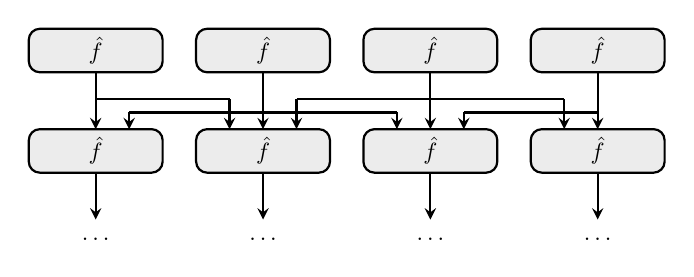
\begin{tikzpicture}[scale=0.85, transform shape]
            % add the Z arrow
            \draw[thick, rounded corners, fill=lightgray!30] (0, 3) rectangle ++ (2, 0.65) node[pos=.5]{$\hat{f}$};
            \draw[thick, rounded corners, fill=lightgray!30] (2.5, 3) rectangle ++ (2, 0.65) node[pos=.5]{$\hat{f}$};
            \draw[thick, rounded corners, fill=lightgray!30] (5, 3) rectangle ++ (2, 0.65) node[pos=.5]{$\hat{f}$};
            \draw[thick, rounded corners, fill=lightgray!30] (7.5, 3) rectangle ++ (2, 0.65) node[pos=.5]{$\hat{f}$};
            %
            \draw[thick, rounded corners, fill=lightgray!30] (0, 1.5) rectangle ++ (2, 0.65) node[pos=.5]{$\hat{f}$};
            \draw[thick, rounded corners, fill=lightgray!30] (2.5, 1.5) rectangle ++ (2, 0.65) node[pos=.5]{$\hat{f}$};
            \draw[thick, rounded corners, fill=lightgray!30] (5, 1.5) rectangle ++ (2, 0.65) node[pos=.5]{$\hat{f}$};
            \draw[thick, rounded corners, fill=lightgray!30] (7.5, 1.5) rectangle ++ (2, 0.65) node[pos=.5]{$\hat{f}$};
            %
            \draw[thick] (1, 2.6) -- (3, 2.6);
            \draw[->, thick, >=stealth] (3, 2.6) -- (3, 2.15);
            \draw[->, thick, >=stealth] (1, 3) -- (1, 2.15);
            %
            \draw[thick] (1.5, 2.4) -- (5.5, 2.4);
            \draw[->, thick, >=stealth] (1.5, 2.4) -- (1.5, 2.15);
            \draw[->, thick, >=stealth] (5.5, 2.4) -- (5.5, 2.15);
            \draw[->, thick, >=stealth] (3.5, 3) -- (3.5, 2.15);
            %
            \draw[thick] (4, 2.6) -- (8, 2.6);
            \draw[->, thick, >=stealth] (4, 2.6) -- (4, 2.15);
            \draw[->, thick, >=stealth] (8, 2.6) -- (8, 2.15);
            \draw[->, thick, >=stealth] (6, 3) -- (6, 2.15);
            %
            \draw[thick] (6.5, 2.4) -- (8.5, 2.4);
            \draw[->, thick, >=stealth] (6.5, 2.4) -- (6.5, 2.15);
            \draw[->, thick, >=stealth] (8.5, 3) -- (8.5, 2.15);
            %
            \draw[->, thick, >=stealth] (1, 1.5) -- (1, 0.8);
            \draw[->, thick, >=stealth] (3.5, 1.5) -- (3.5, 0.8);
            \draw[->, thick, >=stealth] (6, 1.5) -- (6, 0.8);
            \draw[->, thick, >=stealth] (8.5, 1.5) -- (8.5, 0.8);
            %
            \node[] at (1, 0.5) {$\ldots$};
            \node[] at (3.5, 0.5) {$\ldots$};
            \node[] at (6, 0.5) {$\ldots$};
            \node[] at (8.5, 0.5) {$\ldots$};
        \end{tikzpicture}
        \caption{Embedding the computation of space-time for $1$-dimensional first neighbors cellular automaton $A$ into an ultimately periodic configuration of a $2$-dimensional cellular automaton $B$}
        \label{fig:logical-universality}
    \end{figure}
    
\end{proof}


\section{Appendix: Gates Implementation}\label{sec:app-gates}

We can combine our custom delay-insensitive gates to create asynchronous \textsf{NAND} (Figure \ref{fig:nand}) and fan-out (Figure \ref{fig:fan-out}) using dual-rail encoding. To verify the correctness of our construction we have implemented these gates in \texttt{Golly} \cite{golly}, a cellular automaton simulator and observed their space-time evolution. We use $\raisebox{-3.5pt}{\CustomSmall{w}}$ for $0$, $\raisebox{-3.5pt}{\CustomSmall{g}}$ for $1$ and $\raisebox{-3.5pt}{\CustomSmall{b}}$ for $2$ for a more clear representation. 

\begin{figure}[H]
    \centering
    \includegraphics[width=0.25\linewidth]{figures/fan-out.jpg}
    \caption{Implementation of fan-out inside a configuration of cellular automaton $\mathbb{X}$ using dual rail encoding. The input is set to true (the first ``tube'' on the left is colored black making its right neighbor active).}
    \label{fig:fan-out}
\end{figure}

\begin{figure}[H]
    \centering
    \includegraphics[width=0.75\linewidth]{figures/NAND.jpg}
    \caption{Implementation of \textsf{NAND} gate inside a configuration of cellular automaton $\mathbb{X}$ using dual rail encoding. In this case, both inputs are initialized to true (the first and third ``tubes'' on the left are colored black making their right neighbors active).}
    \label{fig:nand}
\end{figure}




\end{document}
